\documentclass[MSc, francais, english]{ulthese}
\selectlanguage{english}

\ifxetex\else \usepackage[utf8]{inputenc} \fi

\usepackage{amsmath}          % recommandé pour les mathématiques
%\usepackage{icomma}           % gestion de la virgule dans les nombres

\usepackage{mathpazo}         % texte et mathématiques en Palatino
\usepackage{mathptmx}         % texte et mathématiques en Times

\usepackage{tabularx,ragged2e}
\renewcommand\tabularxcolumn[1]{>{\Centering}p{#1}}
\usepackage{makecell} % Cell auto line break for table \makecell{bla \\ bla}
\usepackage{graphicx}
\usepackage{subfig}
\usepackage{caption}
\usepackage{color}
\usepackage{siunitx}
%\usepackage{cite} % sort citation numbers automatically
%\usepackage[numbers]{natbib}

\usepackage{hyperref}
\hypersetup{colorlinks,allcolors=ULlinkcolor}
%% Options de mise en forme du mode français de babel. Consulter la
%% documentation du paquetage babel pour les options disponibles.
%% Désactiver (effacer ou mettre en commentaire) si l'option
%% 'nobabel' est spécifiée au chargement de la classe.
%\frenchbsetup{%
    %CompactItemize=false,         % ne pas compacter les listes
    %ThinSpaceInFrenchNumbers=true % espace fine dans les nombres
%}

\newcommand{\todo}[1]{\textcolor{red}{{[\textbf{TODO}: #1]}}}

\usepackage{xspace}
\newcommand{\chapzerotitle}{Literature Review\xspace}
\newcommand{\chaplidartitle}{Snowfall Influence on LiDAR Data\xspace}
\newcommand{\chapslamtitle}{Forest Influence on LiDAR-Based Place Recognition\xspace}
\newcommand{\correspond}{\mathrel{\widehat{=}}}


\usepackage[acronym]{glossaries}
%\renewcommand*{\glstextformat}[1]{\textcolor{black}{#1}} % if link, select color
\renewcommand{\glstextformat}[1]{\textit{#1}} % Make gls word italic

\newacronym{ugv}{UGV}{Unmanned Ground Vehicle}
\newacronym{lidar}{LiDAR}{Light Detection And Ranging}
\newacronym{ptu}{PTU}{Pan-Tilt Unit}
\newacronym{gps}{GPS}{Global Positioning System}
\newacronym{imu}{IMU}{Inertial Measurements Units}
\newacronym{sonar}{SONAR}{Sound Navigation And Ranging}
\newacronym{radar}{RADAR}{Radio Detection And Ranging}
\newacronym{rgb}{RGB}{Red, Green, Blue colour}
\newacronym{rgbd}{RGB-D}{Red, Green, Blue plus Depth}
\newacronym{ndt}{NDT}{Normal Distribution Transform}

\newacronym{3d}{3D}{Three Dimensional}
\newacronym{2d}{2D}{Two Dimensional}
\newacronym{fov}{FOV}{Field Of View}

\newacronym{os}{OS}{Operating System}
\newacronym{ssh}{SSH}{Secure Shell}
\newacronym{gui}{GUI}{Graphical User Interface}
\newacronym{udp}{UDP}{User Datagram Protocol}
\newacronym{ros}{ROS}{Robot Operating System}

\newacronym{slam}{SLAM}{Simultaneous Localization And Mapping}
\newacronym{bow}{BoW}{Bag of Words}
\newacronym{icp}{ICP}{Iterative Closest Point}

\newacronym{fn}{FN}{False Negative}
\newacronym{fp}{FP}{False Positive}
\newacronym{tn}{TN}{True Negative}
\newacronym{tp}{TP}{True Positive}

\makeglossaries


\titre{Robot Perception Using LiDAR for Navigation in Complex Environments}
% \titre{Ceci est un exemple de long titre \\
%   avec saut de ligne manuel}
% \soustitre{Sous-titre le cas échéant}
% \soustitre{Ceci est un exemple de long sous-titre \\
%   avec saut de ligne manuel}
\auteur{Sébastien Michaud}
\programme{Maîtrise en informatique}
\annee{2015}

\begin{document}

\frontmatter

\pagetitre

\chapter*{Résumé}
\phantomsection\addcontentsline{toc}{chapter}{Résumé}

\begin{otherlanguage*}{francais}

    Pour assurer une navigation sécuritaire et efficace, les robots mobiles reposent grandement sur l'utilisation des capteurs embarqués. L'un des capteurs qui est de plus en plus utilisé pour la navigation des robots est le \emph{Light Detection And Ranging} (LiDAR). Il produit de l'information riche sur la structure tridimensionnelle de l'environnement du robot et ce, indépendamment des conditions lumineuses. Bien que les recherches récentes montrent une amélioration des performances de navigation pour des problèmes contraints comme la conduite urbaine dans les conditions ensoleillées de la Californie, faire face à des environnements non-structurés complexes ou des conditions météorologiques difficiles reste problématique. Dans ce mémoire, nous présentons une analyse de l'influence de telles conditions sur la navigation basée sur les LiDARs. Notre première contribution est d'évaluer comment quatre LiDARs couramment utilisés (Velodyne HDL-32E, SICK LMS151, SICK LMS200 et Hokuyo UTM-30LX-EW) sont affectés par les flocons de neige durant des tempêtes de neige. Nous créons un nouvel ensemble de données en faisant l'acquisition de données avec les quatre capteurs simultanément durant six précipitations de neige. Une analyse statistique de ces ensembles de données indique que leurs mesures peuvent être modélisées de manière probabiliste, permettant l'utilisation d'un système bayésien pour améliorer la robustesse. De plus, nous observons l'évolution temporelle de l'impact de la neige durant ces précipitations, et caractérisons la sensibilité de chaque capteur. Finalement, nous concluons que les précipitations de neige ont peu d'influence au-delà de \SI{10}{\meter}. Notre seconde contribution est d'évaluer l'impact de structures tridimensionnelles complexes présentes en forêt sur les performances des algorithmes de navigation. Étant donné que l'habileté à reconnaître des endroits visités est utile à plusieurs problèmes de navigation, nous avons choisi d'effectuer nos expériences avec un algorithme de l'état de l'art en reconnaissance d'endroits. Nous avons acquis des données dans un environnement extérieur structuré et en forêt ainsi qu'avec deux LiDARs (LMS151, HDL-32E). Cela permet d'évaluer l'influence de l'environnement sur les performances de reconnaissance d'endroits, mais aussi celle du capteur choisi. Notre hypothèse est que le plus proche deux balayages laser sont l'un de l'autre, le plus haut le score (i.e. la croyance que ces balayages laser proviennent du même endroit) sera, mais modulé par le niveau de complexité de l'environnement. Nos expériences confirment que la forêt, avec ses réseaux de branches compliqués et son feuillage, produit plus de données aberrantes et induit une chute plus rapide des scores en fonction de la distance que pour les environnements structurés, présent entre des bâtiments. De façon similaire, les scores pour le Velodyne chutes légèrement plus rapidement en fonction de la distance que pour le SICK. Notre conclusion finale est que, les environnements complexes étudiés impactent négativement les performances de navigation basée sur les LiDARs, ce qui devrait être considéré pour développer des algorithmes de navigation robustes.


\end{otherlanguage*}

\chapter*{Abstract} \phantomsection\addcontentsline{toc}{chapter}{Abstract} 

\begin{otherlanguage*}{english}

    To ensure safe and efficient navigation, mobile robots heavily rely on their ability to use on-board sensors to perceive and model their environment. One such sensor increasingly used for robot navigation the \gls*{lidar}, which prove to provided rich information about the three-dimensional structure of the robot surroundings, independent of illumination conditions. Although recent research showed improvement in \gls*{lidar}-based navigation performance for constraint problems such as urban driving in sunny California, dealing with challenging conditions such as unstructured environments or difficult weather conditions remain challenging. In this thesis, we present an analysis of the influence of such complex conditions on \gls*{lidar}-based navigation.

    Our first contribution is to evaluate how four commonly-used \gls*{lidar}s (Velodyne HDL-32E, SICK LMS151, SICK LMS200 and Hokuyo UTM-30LX-EW) are affected by snowflakes during snowstorms. We created a novel dataset by acquiring data from the four sensors simultaneously during 6 snowfalls. Statistical analysis of this dataset indicated that these sensor measurements can be modeled in a probabilistic manner, allowing the use of a Bayesian framework to improve robustness. Moreover, we were able to observe the temporal evolution of the impact of the falling snow during these snowstorms, and characterized the sensitivity of each device. Finally, we concluded that the falling snow had little impact beyond a range of \SI{10}{\meter}.

    Our second contribution is to evaluate the impact of complexity of \gls*{3d} structures in an environment on a navigation algorithm performance. Because the ability to recognize previously-visited places is useful for solving many navigation problems, we choose to perform our experiments using a state-of-the-art place recognition algorithm. Using the SICK LMS151, we acquired a dataset in an environment similar to those used in the original place recognition paper and a dataset in a forest for comparison. We also reproduced the forest dataset using the Velodyne HDL-32E, in order to determine if the sensor influences performance. Analysis of the results was performed using the output of the original place recognition algorithm, which represented the belief that two input scans originate from the same place. Our hypothesis was that the closer two scans were acquired from each other, the higher we expected the score to be, but modulated by the level of complexity of the environments. Our experiments confirmed indeed that the forests, with their intricate network of branches and foliage, produced more outliers and induced place recognition scores to decrease more quickly with distance than for open, structured environment, found between building. Similarly, the scores for the Velodyne decrease slighly faster with distance for the Velodyne than for the SICK. 

\end{otherlanguage*} 

%\cleardoublepage

\tableofcontents
\cleardoublepage

\listoftables
\cleardoublepage

\listoffigures
\cleardoublepage

%\dedicace{Dédicace si désiré}
%\cleardoublepage

%\epigraphe{Texte de l'épigraphe}{Source ou auteur}
%\cleardoublepage

\chapter*{Acknowledgements}
\phantomsection\addcontentsline{toc}{chapter}{Acknowledgements}

Firstly, I would like to express my sincere gratitude to my advisors Prof. Philippe Giguère and Prof. Jean-François Lalonde, for the continuous support during my Master studies. They seamlessly provided funding and research equipment, they assisted me during the writing, but most of all, they shared their precious knowledge and time to help me reach my goals. 

A very special thanks goes out to François Pomerleau, a Postdoctoral Fellow who taught me a lot about the world of research and helped me learn the essential tools for applied robotics. He always answered my numerous questions patiently and provided me with useful tips for my work, even after leaving our research lab.

I would like to thank my fellow labmates for the help they gave me on multiple projects, the stimulating discussions we had and the fun time we shared during social activities.  


\mainmatter

\chapter{Personnal Notes}

Structure for intro
\begin{itemize}
    \item What the topic is about
    \item Niche (why there is need for research on your topic)
    \item Introduce the current research (hypothesis, research question)
\end{itemize}

Elements of the intro
\begin{enumerate}
    \item state the general topic and give some background
    \item provide a review of the literature related to the topic
    \item define the terms and scope of the topic
    \item outline the current situation
    \item evaluate the current situation (advantages/ disadvantages) and identify the gap
    \item identify the importance of the proposed research
    \item state the research problem/ questions
    \item state the research aims and/or research objectives
    \item state the hypotheses
    \item outline the order of information in the thesis
    \item outline the methodology
\end{enumerate}

What is methods:
\begin{itemize}
    \item Information to allow the reader to assess the believability of your results.
    \item Information needed by another researcher to replicate your experiment.
    \item Description of your materials, procedure, theory.
    \item Calculations, technique, procedure, equipment, and calibration plots.
    \item Limitations, assumptions, and range of validity.
    \item Desciption of your analystical methods, including reference to any specialized statistical software.
\end{itemize}

\chapter*{Introduction}         % ne pas numéroter
\phantomsection\addcontentsline{toc}{chapter}{Introduction} % inclure dans TdM

Une thèse ou un mémoire devrait normalement débuter par une
introduction. Celle-ci est traitée comme un chapitre normal, sauf
qu'elle n'est pas numérotée.

\chapter{\chapzerotitle}
\label{chap:literature_review}


\section{Introduction}
Literature review helps understand what was done and determine what is unexplored\dots
We will present general articles related to ugv navigation in outdoor environments, but section X and Y will presents a short literature review more related to the topics of the chapters.


\section{Sensors}
Sensors are the basis of navigation. Sensor characterization, fusion, calibration\dots

~\cite{Bosch2001}:
Review usual lidar techniques (pulsed, phase-shift and frequency modulated continuous wave), basics then limitations.


\section{Features and Machine Learning}
While we will not address this topic specifically, the algorithm used for the place recognition analysis highly depends on the chosen features.  
Bring table about features here if I do. Might want to include the part about tree features discussed in the next section. Put comparative analysis. Tackle DNN.
~\cite{Steder2011a} NARF, ~\cite{Rusu2009} FPFH, ~\cite{Yu2009} ISS, ~\cite{Tombari2010} SHOT, ~\cite{Harris1988} Harris, ~\cite{Lowe2004} SIFT, ~\cite{Bay2006} SURF

~\cite{Filipe2014}:
Comparative evalutation of 3D Keypoint Detectors in RGB-D Obeject dataset. They verify the invariance of the 3D keypoints detectors to rotaions, scales and translation.


\section{SLAM Complex Environments}
Brief overview of slam techniques, section will focus on articles related to place recognition using lidar. Might want to say that we are mainly concern by the forested environments here. 

~\cite{Hussein2015}:
Geolocation of ugv in forest (horizontal position) by finding geometric match between a map of observed tree stems using onboard lidar with a map generated from the structure of thee crowns from high resolution aerial orthoimagery of the forest canopy. No need for a priori knowledge of the area surrounding the robot, only input is the geometry of detected tree stems.

State that 2D solutions for slam pretty much meet our needs, they yield precise results in real time\dots

~\cite{Grisetti2007}: Gmapping,
They use a particle filter to solve SLAM (grid map). Each particle carry an individual map. They take into account the movement but also the most recent observations, which decrease uncertainty. They use selective selective resampling to reduce the problem of particle depletion. They do indoor AND outdoor. 

~\cite{Kohlbrecher2011}: Hector mapping,
Focus on search and rescue. Learn map of unknown environments, occupancy grid, low computational resources. Lidar + IMU. Fast approximation of map gradients and multi resolution grids. Pretend they don't need explicit loop closure\dots


Then they start using 3D, this is more applicable to complex environments (remove some assumptions)

~\cite{Magnusson2009}:
This is NDT. First in my knowledge to do loop closure based on 3D laser scans. Address the problems of greater amount of data (3D vs 2D) and the 3D rotation invariance. NDT surface representation to create feature histograms based on the surface orientation and smoothness (this compress data). Rotation invariance via alignment of dominant surface orientations.

~\cite{Song2012}:(might be good to cite original ICP or review from F. Pomerleau)
They proposes a localisation solution in forested environments. They use the largest group of approximately parallel tree trunk features to align successive scans along five dimensions (except z). Optimal transformation determined based on the axes of two tree pairs. Then they align ground by minimizing the differences of points shared in the cells. (they basically do ICP, but they pretend to remove problems such as initial transformation and noisy scene.) (This is high level engineered features, could use this for smooth transition in the text)

~\cite{Iagnemma2012}:
The method used in the previous article to extract tree truck parameters from point cloud. 3 purely geometric steps: First, the raw point clouds are segmented by utilizing the circular shape of trees, and segments are grouped into tree sections based on the principle of spatial proximity. Second, circles and axes are extracted from tree sections which are subject to loss of shape information. Third, by clustering and integrating the tree sections resulted from various space inconsistencies, straight tree trunk landmarks are finally formed for future localization. The experimental results from real forested environments are presented.

~\cite{Mcdaniel2012}:
Article that segment ground and trees that I used at the beginning of my master. 

~\cite{Lalonde2006}:
J-F Lalonde article about vegetation classification using eigenvalues/vectors. 

~\cite{Wurm2009}:
This paper present a technique that use laser remission values to detect grass like vegetation. They use a self-supervised classifcation vibration based. 

~\cite{Besl1992}:
Original ICP article

~\cite{Colas2013}:
Article doing path planning in complex environments for search and rescue based on ICP for 3D terrains. 

~\cite{Pomerleau2013}:
This article present an analysis of ICP variants for real world applications. They also propose an open-source icp library that operate in real time.  

~\cite{Pomerleau2015a}:
A Review of Point Cloud Registration Algorithms for Mobile Robotics\dots


\begin{table}[H]
    \centering
    \begin{tabular}{@{}llll@{}}
        \toprule
        \textbf{Type of data}  & \textbf{Keypoint/descriptor} & \textbf{Name}               & \textbf{Reference} \\
        \hline
        Image                  & Keypoint                     & Harris and Stephens corners & \cite{Harris1988}  \\
        Image                  & Both                         & SIFT                        & \cite{Lowe2004}    \\
        Image                  & Both                         & SURF                        & \cite{Bay2006}     \\
        \gls*{3d}              & Descriptor                   & FPFH                        & \cite{Rusu2009}    \\
        \gls*{3d}              & Both                         & ISS                         & \cite{Yu2009}      \\
        \gls*{3d}              & Descriptor                   & SHOT                        & \cite{Tombari2010} \\
        \gls*{3d}              & Both                         & NARF                        & \cite{Steder2011a} \\
        \bottomrule
    \end{tabular}
    \caption{Examples of popular descriptors and keypoints detectors for images and \gls*{3d} data. Some \gls*{2d} keypoints have been adapted for \gls*{3d} such as Harris and Stephens and SIFT.}
    \label{tab:features_examples}
\end{table}

\chapter{LiDAR Characterization}

\begin{itemize}
    \item What is a LiDAR (Useful for more precise,)
    \item How it works
    \item Why is it useful in robotics (visual vs geometrical info)
\end{itemize}

\chapter*{Introduction}         % ne pas numéroter
\phantomsection\addcontentsline{toc}{chapter}{Introduction} % inclure dans TdM

Une thèse ou un mémoire devrait normalement débuter par une
introduction. Celle-ci est traitée comme un chapitre normal, sauf
qu'elle n'est pas numérotée.

\section{Data Acquisition}
\label{sec:chap_slam_data_acquisition}

In the following section, we first describe the robotic platform and sensors used to gather our place recognition dataset. We then describe in more details the dataset acquisition procedure and the resulting data.


\subsection{Robotic Platform}
\label{ssec:chap_slam_platform}

The Husky A200 is a medium size (\SI{990 x 670 x 390}{\milli\meter}) \gls*{ugv} developed by \cite{ClearpathWeb}. It is a rugged robot designed for all terrain conditions, therefore well suited for our experiments in the forest. It uses a differential-drive skid steer allowing easy control and in place turns for our data acquisition. It has a maximum speed of \SI{1}{\meter\per\second}, but we generally acquire data at a lower speed to minimize odometry and range data errors. This platform, with a maximum payload capability of \SI{75}{\kilo\gram}, can easily carry all sensors used for our experiments. Our platform is shown in Figure~\ref{fig:chap_slam_husky}. More details about the available devices are presented in Table~\ref{tab:husky_devices}.

\begin{figure}[H]
    \centering
    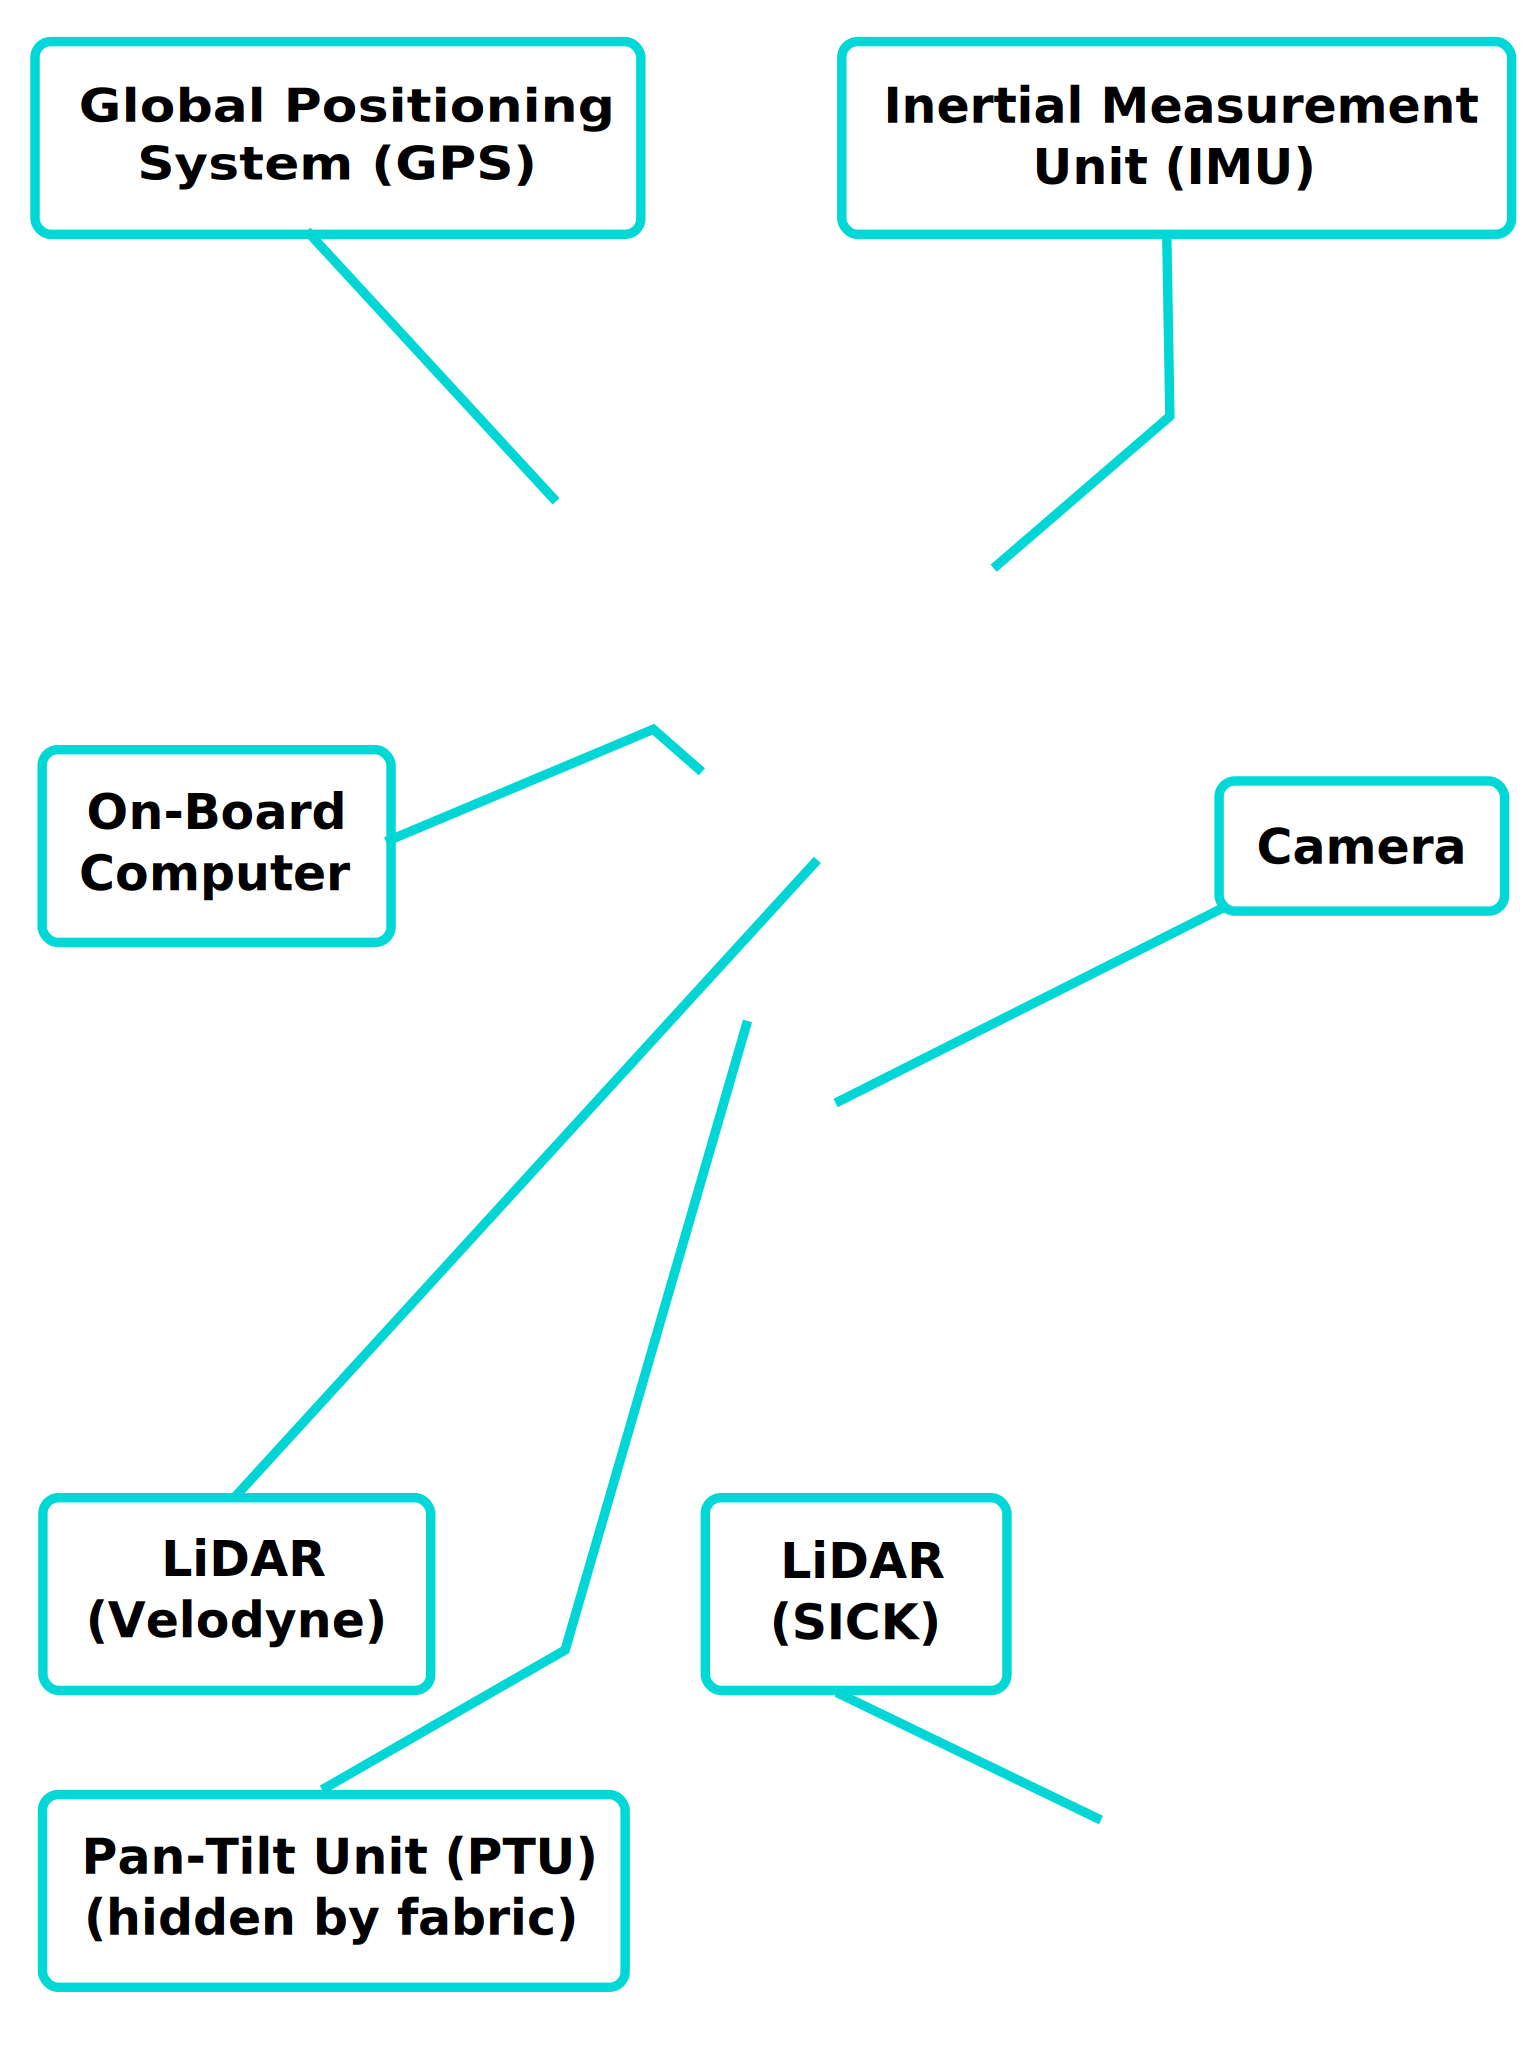
\includegraphics[width=0.98\linewidth]{img/chap_slam/husky_labelled.png}
    \caption{The robotic platform (Husky A200) and the devices used for data acquisition. The SICK \gls*{lidar} is not mounted, but is shown on the bottom right corner of the figure. Note that the \gls*{ptu} is hidden by a cover and the on-board computer is mostly occluded by the Velodyne \gls*{lidar}.}
    \label{fig:chap_slam_husky}
\end{figure}

\begin{table}[H]
    \centering
    \begin{tabular}{@{}llll@{}}
        \toprule
        \textbf{Device} & \textbf{Manufacturer}       & \textbf{Model}  & \textbf{Use}                          \\ \hline
        Computer        & --                          & --              & Data acquisition/synchronisation      \\
        Gateway         & Microhard System Inc.       & VIP2400         & Network and Wi-Fi communication       \\
        Gamepad         & Logitech                    & F710            & Remote control of the robot movements \\
        \gls*{lidar}    & Velodyne                    & HDL-32E         & Point cloud acquisition               \\
        \gls*{lidar}    & SICK                        & LMS151          & Point cloud acquisition               \\
        \gls*{ptu}      & FLIR Motion Control Systems & D46-17          & Rotate the SICK \gls*{lidar}          \\
        \gls*{imu}      & ChRobotics                  & UM6             & Odometry                              \\
        Camera          & Axis                        & M1013           & Visual reference                      \\
        \gls*{gps}      & NovAtel                     & SMART6          & Not used                              \\
        \bottomrule
    \end{tabular}
    \caption{List of devices available on the Husky A200 and their use in our experiments. Note that both \gls*{lidar}s were never mounted at the same time.}
    \label{tab:husky_devices}
\end{table}

The on-board computer (2.4 GHz Intel i5-520M) is an essential element of our experiments, as it connects all devices, acts as a control interface for the robot and stores the acquired data. The computer does not provide a \gls*{gui}, but it is connected to the gateway that broadcasts a WiFi network, allowing \gls*{ssh} communication. The platform is also equipped with a wireless gamepad, which enables manual control of the movements of the robot. Point clouds acquisition is possible using either the SICK LMS151 or the Velodyne HDL-32E. The selected sensor is mounted on the \gls*{ptu}, which remains fixed for the Velodyne, but is rotated with the SICK to merge multiple \gls*{2d} scans into a single \gls*{3d} point cloud. Section~\ref{ssec:chap_slam_platform} gives more details about the resulting point clouds for each sensor.

The sensors described above are essential for our place recognition research, but we also use the wheel encoder along with the \gls*{imu} for odometry estimation and the camera for visual reference of the dataset. Note that we do not use the \gls*{gps}, as we do not want to depend on it for the task of place recognition.


\subsection{Dataset Description}
\label{ssec:chap_slam_platform}

Data acquisition was performed using \gls*{ros}, a set of software libraries and tools created to simplify the development of robotics applications. It provides all drivers for the Husky and our sensors out of the box. Its data publishing system provides timestamps that allows easy synchronization between sensors. The recording tool (rosbag) was used to create our datasets, with data processing performed \textit{a posteriori}.

We produced datasets in two different areas of the Laval University campus. An aerial overview of the path followed by the robot at these two locations is presented in Figure~\ref{fig:chap_slam_path}.

The first site was chosen for its more structured nature and is located between the Alexandre-Vachon and the Adrien-Pouliot buildings. This environment is mostly open, the terrain is smooth and flat and the site contains man-made objects such as buildings, stairs or tables. Examples of pictures acquired by the robot on this site are presented in Figure~\ref{fig:slam_view_building1} and~\ref{fig:slam_view_building2}. This dataset closely resembles the kind of data on which several place recognition algorithms are typically tested on (e.g Freiburg Campus 360 degree 3D scans~\citep{FreiburgDataset}, Robotic 3D Scan Repository~\citep{Datasets}). We will use this data to validate our method.

The second site, chosen for its unstructured nature, is located in a wooded area, also on the Laval University campus. The dataset path starts on a pedestrian walkway, but after its second turn (of approximately \SI{330}{\degree}), it continues for around \SI{100}{\meter} in rougher terrain. This forested environment presents multiple small structures and a lot of occlusions. Figure~\ref{fig:slam_view_forest1} and Figure~\ref{fig:slam_view_forest2} show pictures from the robot camera at this location. This dataset will allow us to better understand the influence of a less structured environment on the place recognition algorithm. In particular, the absence of large flat surfaces and corners typical of buildings, as well as the closeness of the space, will be challenging for place recognition algorithms.

\begin{figure}[H]
    \centering
    \subfloat[]{\label{fig:path_overview}}{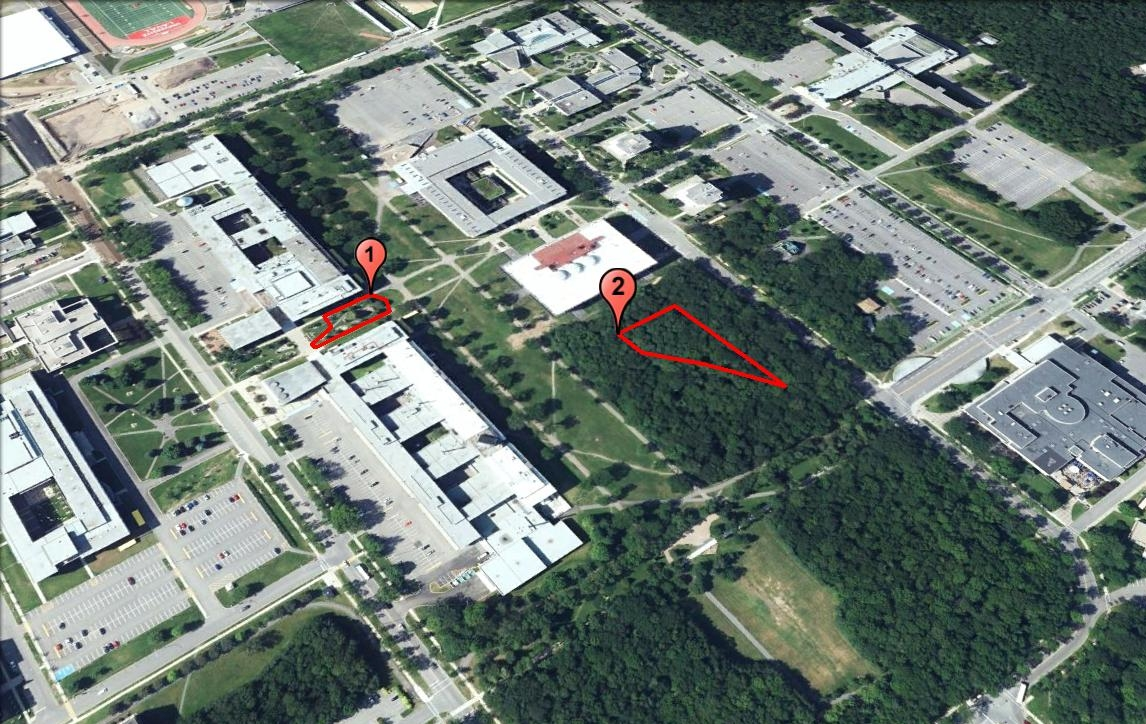
\includegraphics[width=0.995\linewidth]{img/chap_slam/paths.jpg}}\\ \vspace{3mm}
    \subfloat[]{\label{fig:path_building}}{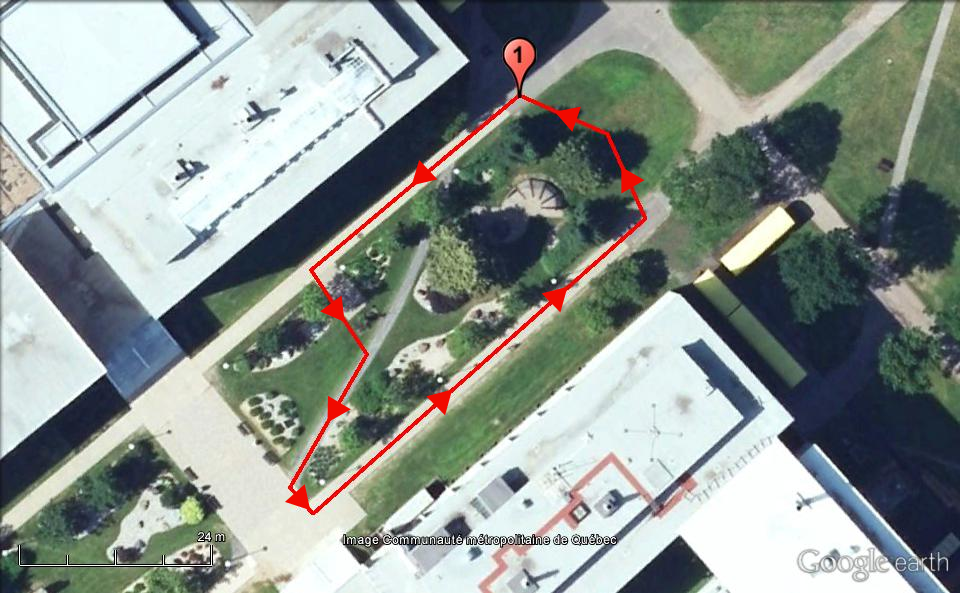
\includegraphics[width=0.485\linewidth]{img/chap_slam/path_building_arrow.png}} \hspace{2mm}
    \subfloat[]{\label{fig:path_forest}}{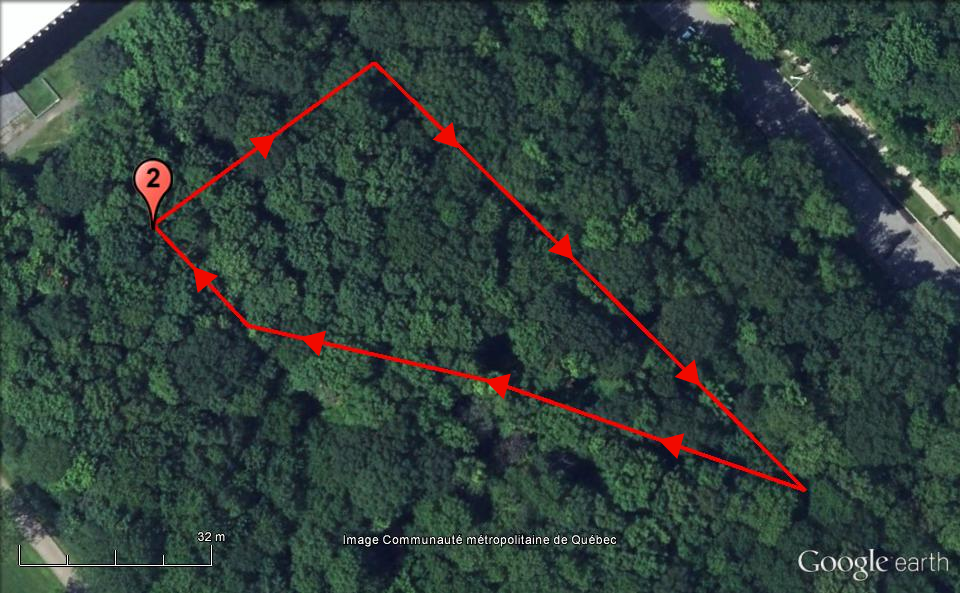
\includegraphics[width=0.485\linewidth]{img/chap_slam/path_forest_arrow.png}}
    \caption{\protect\subref{fig:path_overview} Partial aerial view of the Laval University campus including the two approximate paths followed by the robot for data acquisition. \protect\subref{fig:path_building} Zoomed view of the path followed (counterclockwise from tag 1) in a structured environment. The length of this path is approximately \SI{160}{\meter}. \protect\subref{fig:path_forest} Zoomed view of the path followed (clockwise from tag 2) to create the forest dataset. The length of this path is approximately \SI{275}{\meter}. Images source: Google Earth, (2015)}
    \label{fig:chap_slam_path}
\end{figure}

\begin{figure}[H]
    \centering
    \subfloat[]{\label{fig:slam_view_building1}}{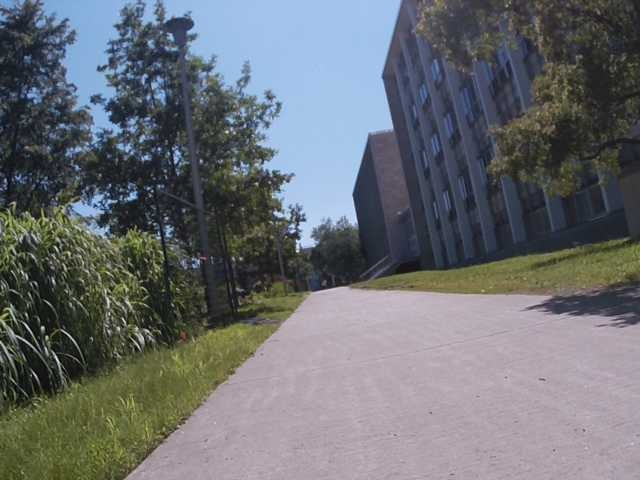
\includegraphics[width=0.47\linewidth]{img/chap_slam/building_view1.jpg}} \hspace{2mm}
    \subfloat[]{\label{fig:slam_view_building2}}{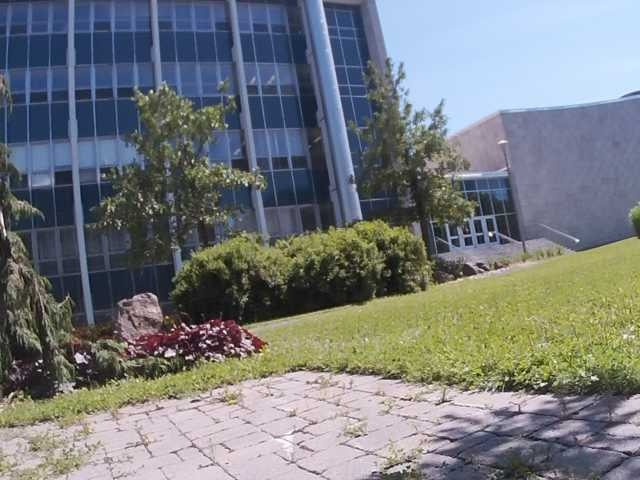
\includegraphics[width=0.47\linewidth]{img/chap_slam/building_view2.jpg}}
    \subfloat[]{\label{fig:slam_view_forest1}}{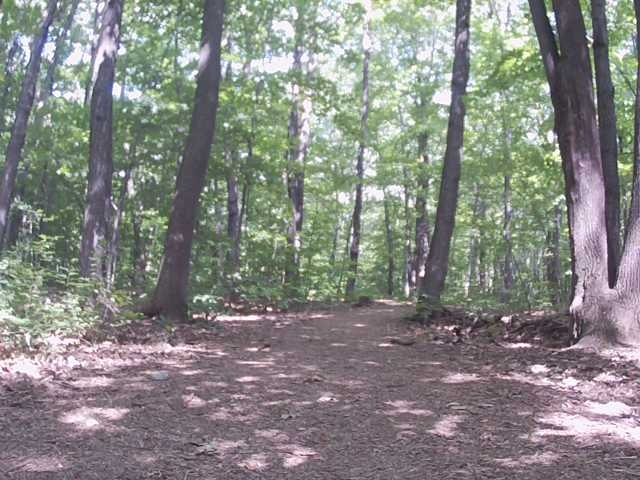
\includegraphics[width=0.47\linewidth]{img/chap_slam/forest_view1.jpg}} \hspace{2mm}
    \subfloat[]{\label{fig:slam_view_forest2}}{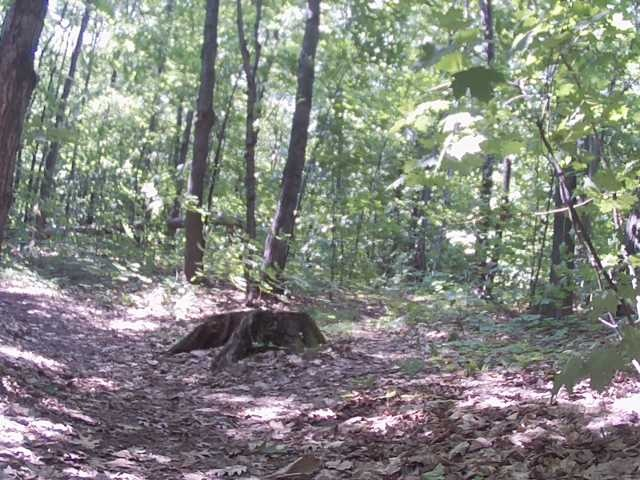
\includegraphics[width=0.47\linewidth]{img/chap_slam/forest_view2.jpg}}
    \caption{Images from the \gls*{ugv} camera during the acquisition of the structured dataset \protect\subref{fig:slam_view_building1} \protect\subref{fig:slam_view_building2} and the unstructured dataset \protect\subref{fig:slam_view_forest1} \protect\subref{fig:slam_view_forest2}.}
    \label{fig:slam_views}
\end{figure}

Besides the influence of the type of environment, we are also interested in the impact of the sensor used and data associated with it. For this analysis, we used two sensors, namely the SICK and the Velodyne, for which you can find details in Table~\ref{tab:slam_sensor_resolution}.

The SICK is a \gls*{2d} \gls*{lidar} with a scanning angle of \SI{270}{\degree}, a resolution of \SI{0.5}{\degree} and an acquisition frequency of \SI{50}{\hertz}. This sensor was placed on the \gls*{ptu} so that the dead angle faced downward. During acquisition, it was rotated around the vertical axis (pan) at a speed of \SI{14.32}{\degree\per\second} for half a turn, while the vehicle was stationary. This procedure allowed the acquisition of 628 \gls*{2d} scans of \SI{540}{\points}, later merged into a single \gls*{3d} point cloud.

The Velodyne, for its part, directly allows \gls*{3d} point cloud acquisition by spinning 32 lasers around its vertical axis. These lasers are evenly distributed between \SI{-30.67}{\degree} and \SI{10.67}{\degree} relative to the horizontal plane. According to the Velodyne datasheet (\cite{VelodyneDatasheet}), the device acquires approximately \SI{700000}{\points\per\second} and publishes at \SI{10}{\hertz}, therefore creating point clouds of \SI{70000}{\points}. Note that these point counts are variable as the rotation speed can change slightly and the use of the \gls*{udp} can lead to some loss of points.

Table~\ref{tab:slam_sensor_resolution} summarizes information about the sensors resolution and \gls*{fov} while Table~\ref{tab:slam_datasets} details the acquisition date and \gls*{lidar} sensor used for each of our datasets.

\begin{table}[H]
    \centering
    \begin{tabular}{@{}lrrrrr@{}}
        \toprule
    \makecell[lc]{\textbf{Sensor}}& \makecell[cc]{\textbf{Horizontal}\\\textbf{resolution}} & \makecell[cc]{\textbf{Vertical}\\\textbf{resolution}} & \makecell[cc]{\textbf{Minimum}\\\textbf{angle}} & \makecell[cc]{\textbf{Maximum}\\\textbf{angle}} & \makecell[cc]{\textbf{Point}\\\textbf{counts}} \\
        \hline
        SICK LMS151      & \SI{0.57}{\degree} & \SI{0.5}{\degree}  & \SI{-45.00}{\degree}  & \SI{90.00}{\degree}  & 339120 \\
        Velodyne HDL-32E & \SI{0.16}{\degree} & \SI{1.33}{\degree} & \SI{-30.68}{\degree}  & \SI{10.67}{\degree}  & 72000  \\
        \bottomrule
    \end{tabular}
    \caption{Details about the point clouds created with our two \gls*{lidar}s. The minimum and maximum angles are given relative to an horizontal plane in the sensor frame of reference and both sensors report \SI{360}{\degree} around the vertical axis. The point counts represent the maximum number of points in the resulting point cloud.}
    \label{tab:slam_sensor_resolution}
\end{table}

\begin{table}[H]
    \centering
    \begin{tabular}{@{}lll@{}}
        \toprule
        \textbf{Site}  & \textbf{Sensor}   & \textbf{Date}                     \\
        \hline
        Structured     & SICK LMS151       & July 16\textsuperscript{th}, 2015 \\
        Unstructured   & SICK LMS151       & July 14\textsuperscript{th}, 2015 \\
        Unstructured   & Velodyne HDL-32E  & May 28\textsuperscript{th}, 2015  \\
        \bottomrule
    \end{tabular}
    \caption{Datasets acquired for place recognition analysis.}
    \label{tab:slam_datasets}
\end{table}

Examples of point clouds from our datasets are shown in Figure~\ref{fig:slam_pointclouds}. We observe that the unstructured environment is more congested and objects are closer to the sensor than for the structured environment. In fact, the average distance of points from the sensor in the unstructured environment is \SI{7.61}{\meter} compared to \SI{9.23}{\meter} for the structured environment. There is also more space without obstacle in the sensor range for the structured dataset. The percentage of points return using the SICK is \SI{82.6}{\percent} on average in the forest dataset compared to \SI{40.2}{\percent} in the structured dataset. These point clouds also illustrate the higher vertical resolution and larger \gls*{fov} of the SICK compared to the Velodyne. The influence of these factors will be discussed in Section~\ref{sec:chap_slam_results}.

\begin{figure}[H]
    \centering
    \subfloat[]{\label{fig:slam_pointcloud_building1}}{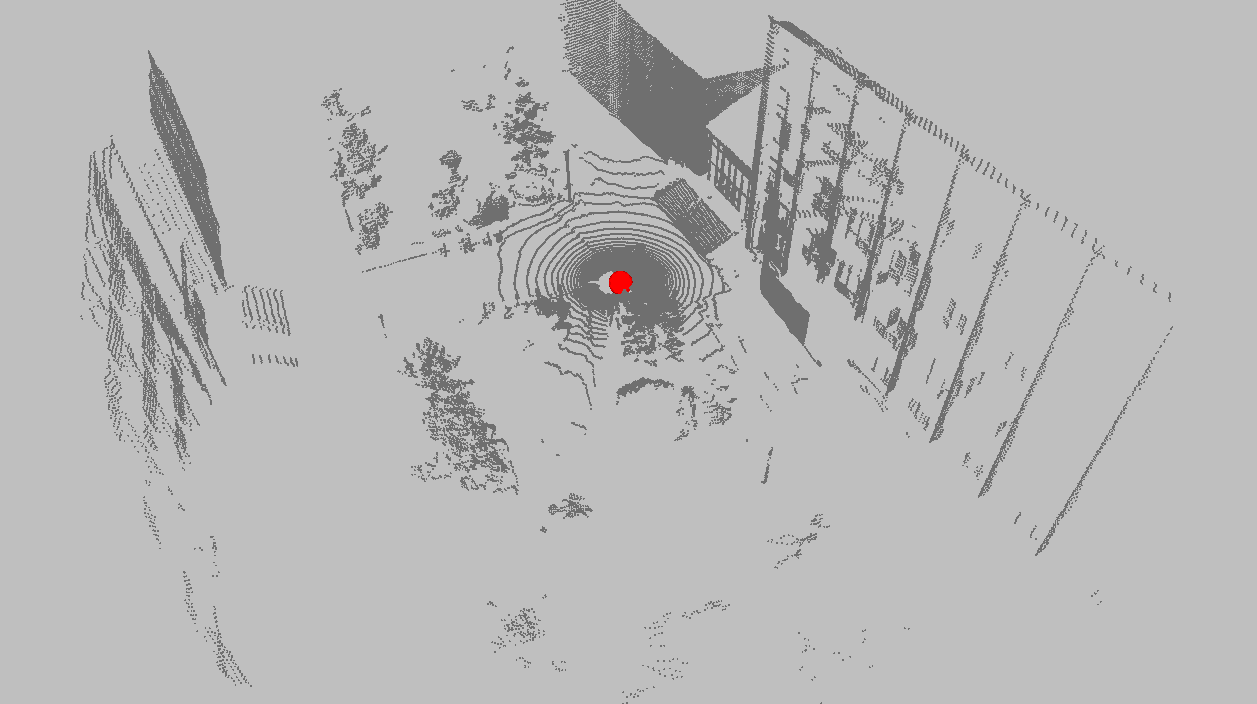
\includegraphics[width=0.47\linewidth]{img/chap_slam/pointcloud_building1.png}} \hspace{2mm}
    \subfloat[]{\label{fig:slam_pointcloud_building2}}{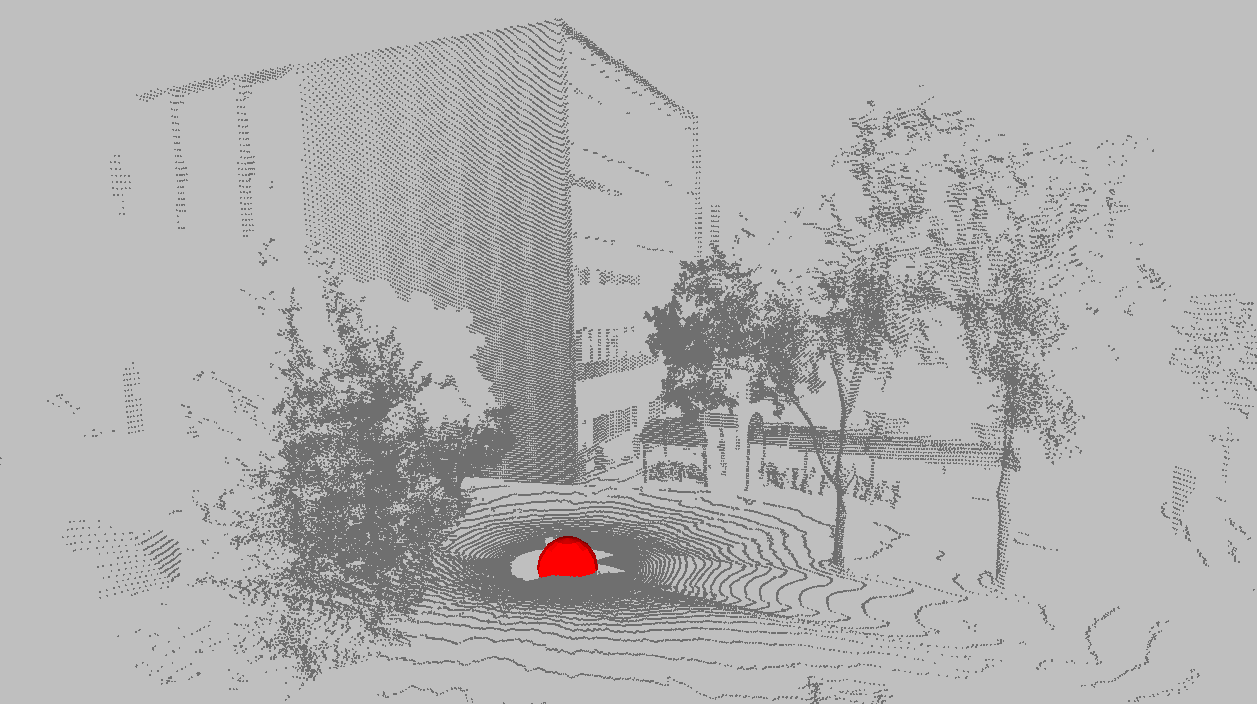
\includegraphics[width=0.47\linewidth]{img/chap_slam/pointcloud_building2.png}}
    \subfloat[]{\label{fig:slam_pointcloud_forest1}}{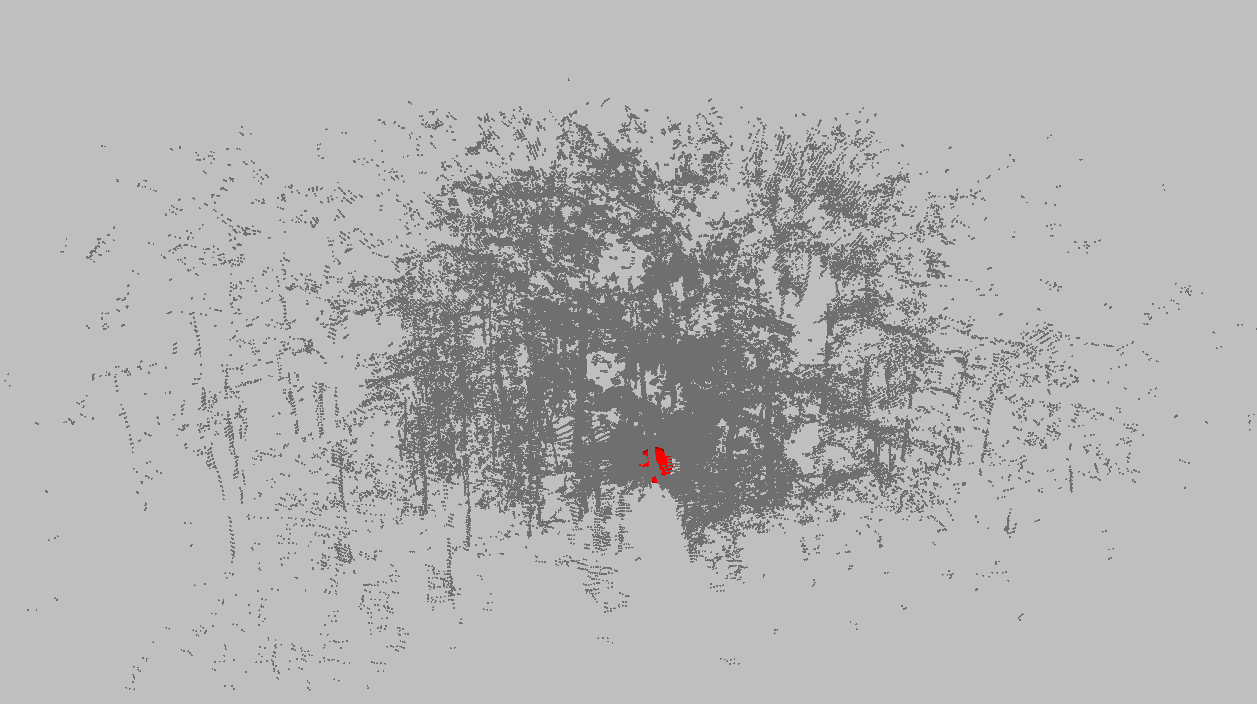
\includegraphics[width=0.47\linewidth]{img/chap_slam/pointcloud_forest1.png}} \hspace{2mm}
    \subfloat[]{\label{fig:slam_pointcloud_forest2}}{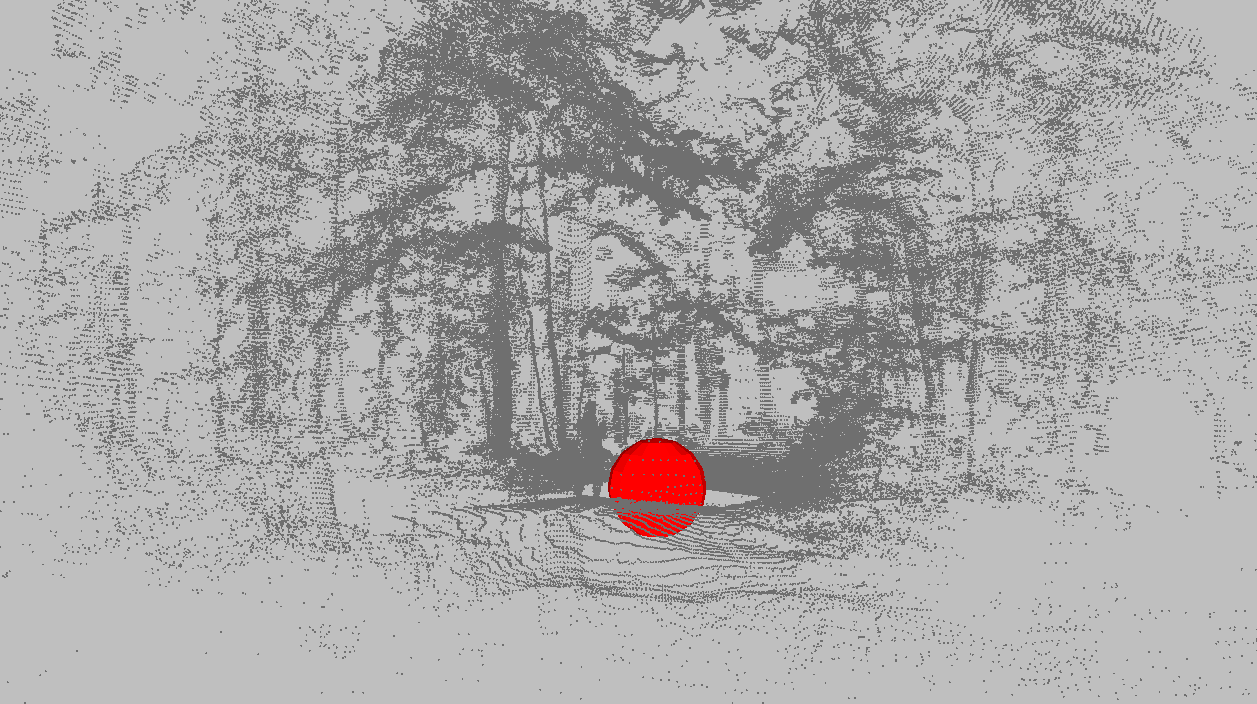
\includegraphics[width=0.47\linewidth]{img/chap_slam/pointcloud_forest2.png}}
    \subfloat[]{\label{fig:slam_pointcloud_velodyne1}}{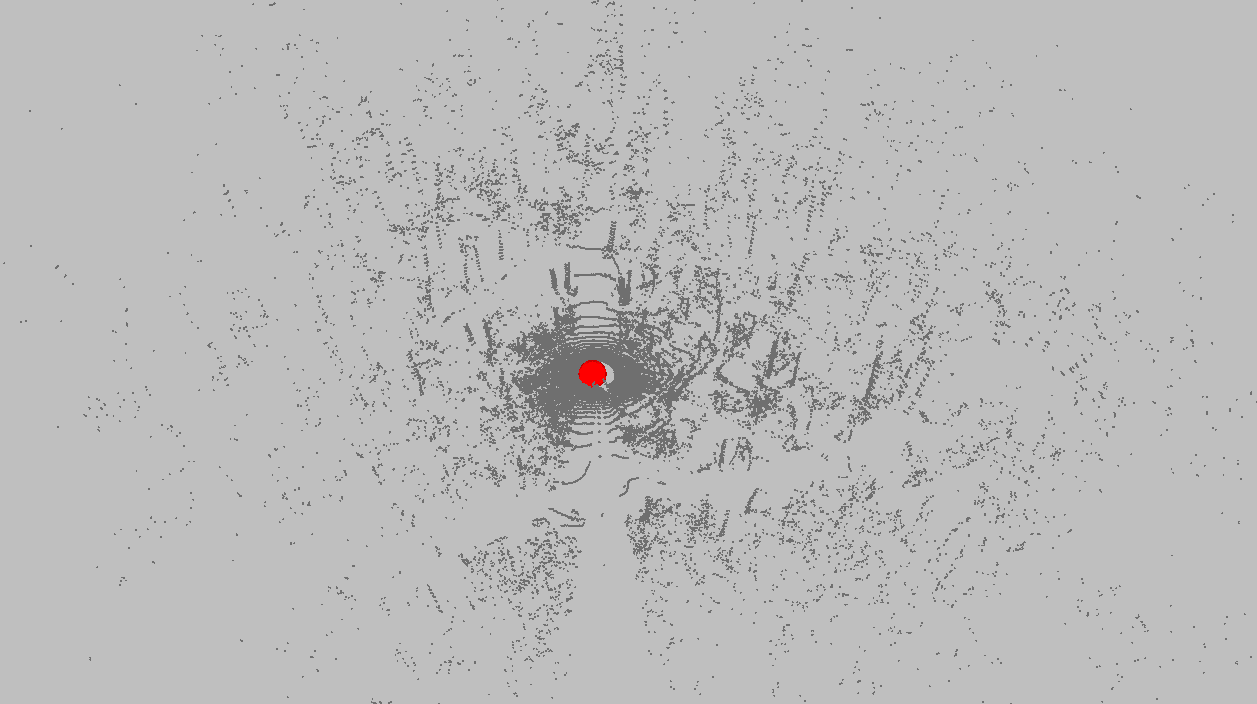
\includegraphics[width=0.47\linewidth]{img/chap_slam/pointcloud_velodyne1.png}} \hspace{2mm}
    \subfloat[]{\label{fig:slam_pointcloud_velodyne2}}{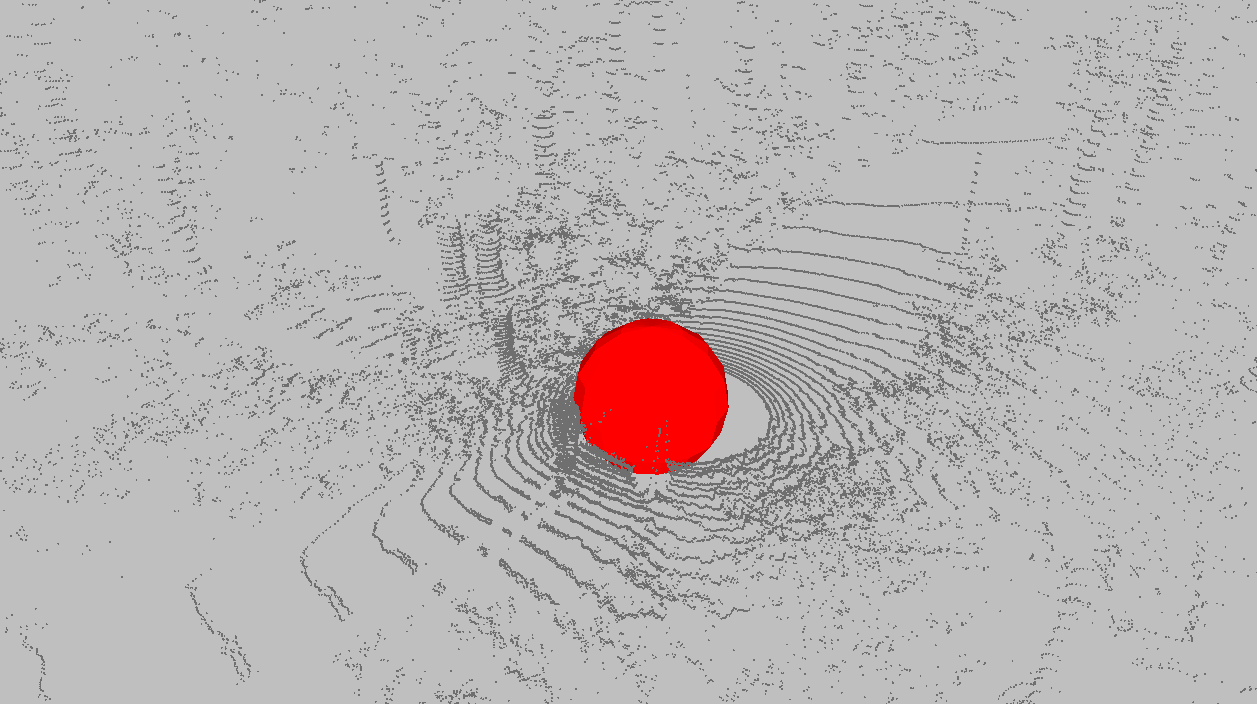
\includegraphics[width=0.47\linewidth]{img/chap_slam/pointcloud_velodyne2.png}}
    \caption{Examples of point clouds from our datasets viewed from different perspectives. \protect\subref{fig:slam_pointcloud_building1} and \protect\subref{fig:slam_pointcloud_building2} show acquisition from the SICK in the structured environment. \protect\subref{fig:slam_pointcloud_forest1} and \protect\subref{fig:slam_pointcloud_forest2} also show point clouds from the SICK, but in the unstructured environment. Finally, \protect\subref{fig:slam_pointcloud_velodyne1} and \protect\subref{fig:slam_pointcloud_velodyne2} show the result of acquisition from the Velodyne in the unstructured environment. Robot position is represented by a red sphere with a \SI{1}{\meter} radius in each picture.}
    \label{fig:slam_pointclouds}
\end{figure}


\section{Temporal Analysis}
\label{sec:chap_lidar_temporal}

In this section, we analyze the temporal behavior of the four sensors for the duration of six complete snowstorms. In particular, we are interested in seeing how the fraction of echoes in snowflakes evolves over time, for all four sensors. First, we will discuss the highly dynamical nature of snowstorms. This will be exemplified by how consecutive scans can have significant quantitative and spatial differences in the distributions of the snowflakes echoes, which justify the use of averaging windows for our analysis. We will then present the actual temporal evolution of these statistics in the form of graphs for all four sensors, and finally briefly discuss the results for each sensor.

\subsection{Extraction of Temporal Statistics}

Snowstorms are highly dynamic processes, with large variation in snowfall rates over their durations. Moreover, the snow physical characteristics (size, shape or reflectance) might vary significantly during a storm, affected by ambient conditions such as humidity level and temperature. Also, wind gusts might pull snow back up in the air or drive it sideways, affecting its effective fall rate. Consequently, one expects during a snowstorm to see significant short, medium and long term variations in the fraction of LiDAR echoes corresponding to the falling snow.

Computing and reporting the temporal statistics for every scan would put too much emphasis on the very short-term statistics. Indeed, the inter-scan variation in the fraction of snowflake echoes can be significant. To better illustrate this point, we have overlaid four consecutive scans in the same plot for the LMS200 and for the first echo returned by the multi-echo Hokuyo sensor in Figure~\ref{fig:LMS200_4Scans_Feb19}, for an intense snowing episode from the 02-19 dataset (see Table~\ref{tab:overview-dataset}). In these figures, we can see strong variations in the fraction of snowflake echoes and their spatial distribution, which we believe can be best described as a random process. One can readily see the fluctuation in these fractions as reported in the brackets of the legend in Figure~\ref{fig:LMS200_4Scans_Feb19}.

To smooth out these fluctuations, statistics are extracted from a number of consecutive scans contained in a time window of around 1~minute (detailed values in Table~\ref{tab:selectionScans}). Figure~\ref{fig:TimingSnow} shows this smoothed fraction of snowflake echoes compared to all returned laser measurements as a function of time, for the six snowiest days of our dataset. To allow for better visualization, only the LMS200 and the Hokuyo's first echo are plotted at their actual scale (1x): Others have been scaled up (from 30x to 200x), with their corresponding scaling factors reported in the legend. As will be shown below, some sensors were much more sensitive than others.

\begin{figure}
    \centering
    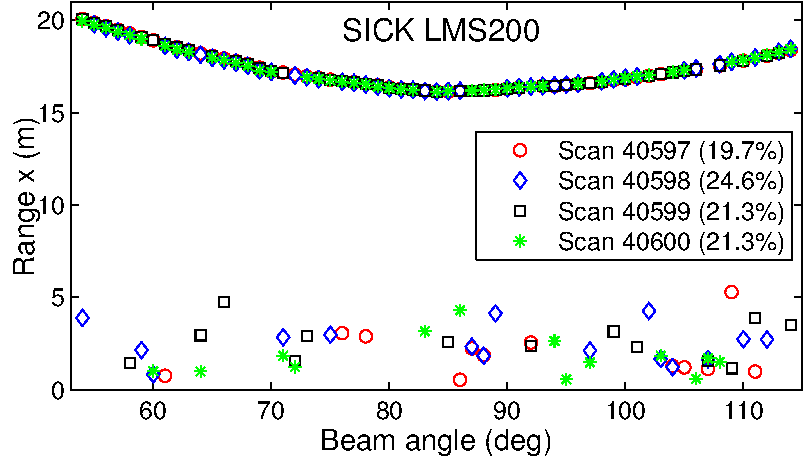
\includegraphics[trim={0.2cm 0 0 0},clip,width=0.7\linewidth]{./img/chap_lidar/LMS200_4Scans_Feb19.pdf}
    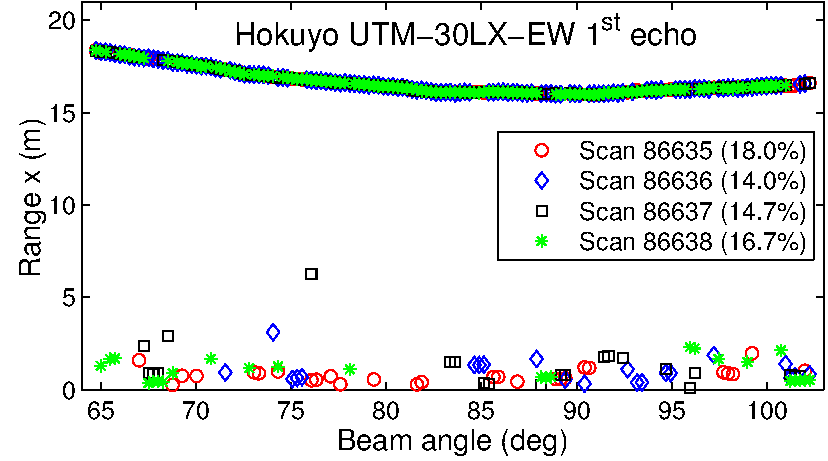
\includegraphics[trim={0.2cm 0 0 0},clip,width=0.7\linewidth]{./img/chap_lidar/Hokuyo_4Scans_Feb19.pdf}
    \caption[Four overlaid consecutive scans for the LMS200 sensor, and the first echo scans for the Hokuyo sensor.]{Four overlaid consecutive scans for the LMS200 sensor (top), and the first echo scans for the Hokuyo sensor (bottom), taken from the 02-19 dataset. Each symbol corresponds to a particular scan. The curved line at the top corresponds to the snow surface on the ground. One can see the rapid variation of the snowflake echoes between scans, and how they are mostly limited to a range $x<\SI{5}{\meter}$. The percentages (in brackets) are the proportion of those echoes in the snowflakes.}
    \label{fig:LMS200_4Scans_Feb19}
\end{figure}

\subsection{Detailed Analysis, per Sensor}

\subsubsection{SICK Sensors LMS200 and LMS151}
Our first conclusion based on Figure~\ref{fig:TimingSnow} is that the most sensitive device was the older LMS200, first introduced in the mid-2000s. For the most intense snowstorms (Figure~\ref{fig:TimingSnow}. b) 02-19, d) 03-17, e) 03-21 and f) 03-30), it peaked at around 15\% of measurements triggered by the falling snowflakes, for averaging windows of \SI{106}{\second}. As an older-generation device, it probably uses less sophisticated algorithms and sensing, and was not directly targeted for harsh outdoor environments. Indeed, its technical description~\citep{LMS200Manual} indicates that ``Raindrops and snow-flakes are cut out using pixel-oriented evaluation'', but this seems only applicable to obstacle detection (field computation), not the actual measurements. No further details are given. On the other hand, the more recent SICK LMS151 exhibits much less sensitivity to snowflakes: The reduction factor for the fraction of snowflakes echoes is in the order of 200-300, granting this device a much higher immunity in snowstorms. Indeed, the highest peak was around 0.1 \% of echoes in snowflakes during the 02-19 dataset. In some sense, this is not surprising considering that the documentation from the manufacturer mentions that this model is targeted for ``all weather conditions''~\citep{LMS151Manual}.


\begin{figure}
    \centering
    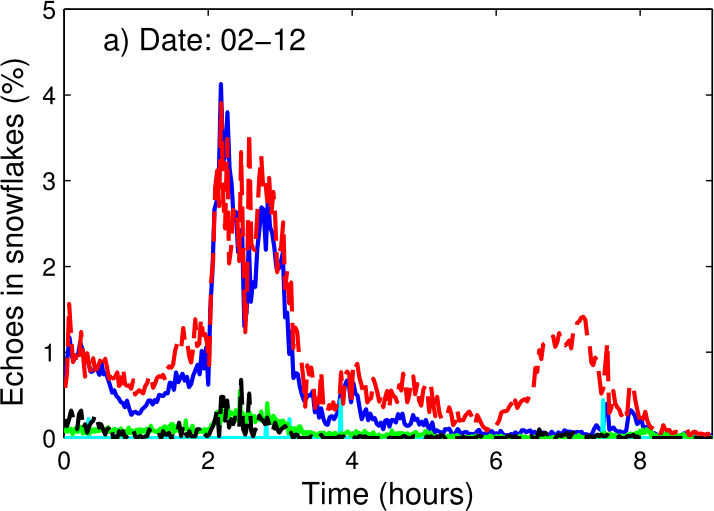
\includegraphics[width=0.45\linewidth]{./img/chap_lidar/timings_cropped_a.png}
    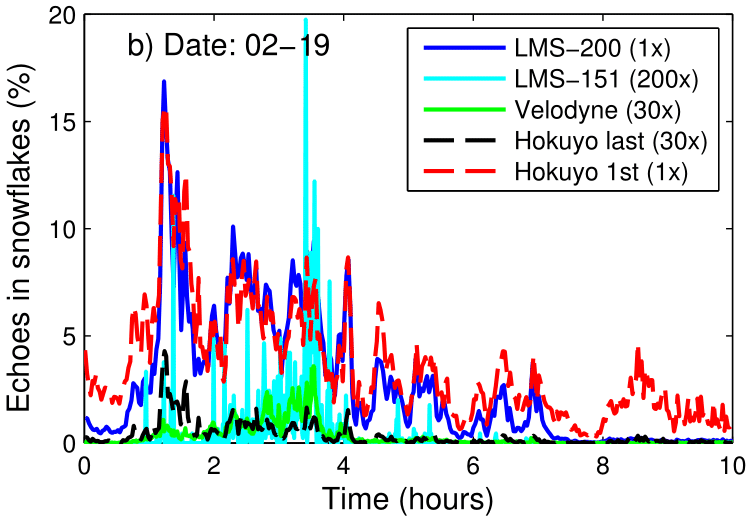
\includegraphics[width=0.45\linewidth]{./img/chap_lidar/timings_cropped_b.png}
    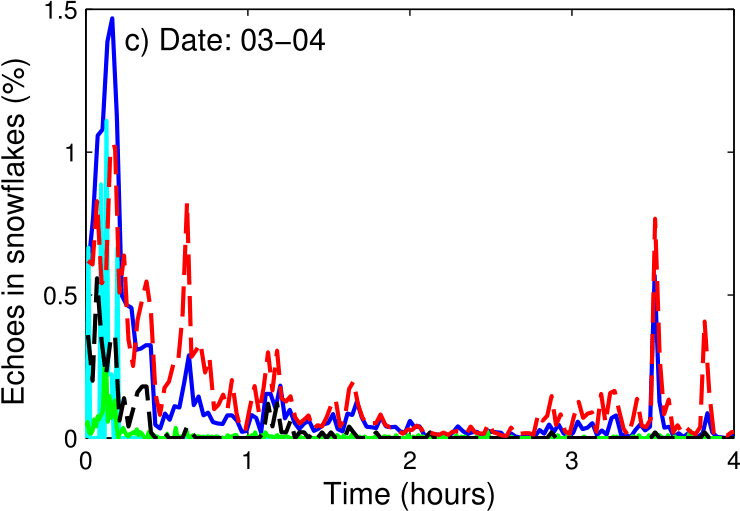
\includegraphics[width=0.45\linewidth]{./img/chap_lidar/timings_cropped_c.png}
    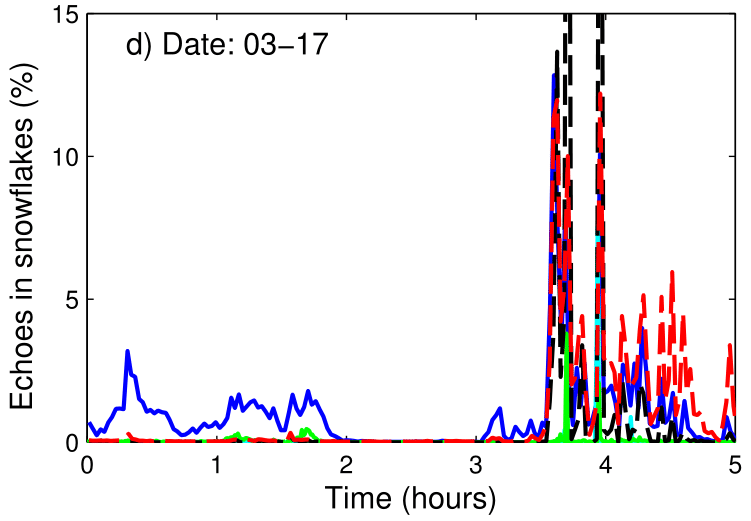
\includegraphics[width=0.45\linewidth]{./img/chap_lidar/timings_cropped_d.png}
    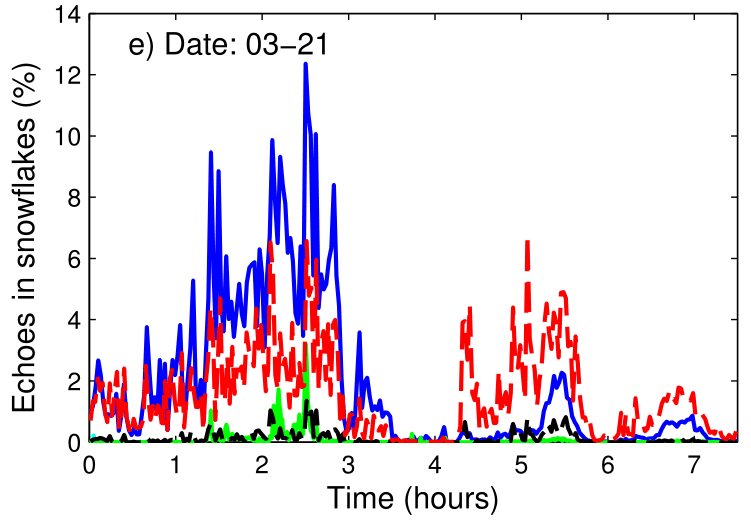
\includegraphics[width=0.45\linewidth]{./img/chap_lidar/timings_cropped_e.png}
    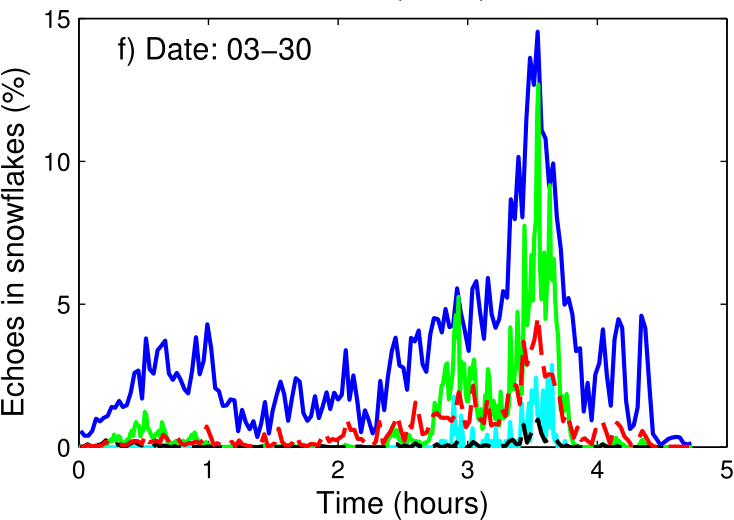
\includegraphics[width=0.45\linewidth]{./img/chap_lidar/timings_cropped_f.png}
    \caption[Temporal evolution of the percentage of echoes coming from the falling snow within \SI{5}{\meter} of the sensors during the 6 most intense snowfall episodes.]{Temporal evolution of the percentage of echoes coming from the falling snow (range $x<$\SI{5}{\meter}) during the 6 most intense episodes, for all 4 sensors. The data is smoothed by taking statistics for small time windows. Except for the LMS200 and Hokuyo first echo, all other sensors statistics have been scaled up (factor in bracket of legend b) for ease of visual comparison. Time is in hour, starting from the beginning of the data capture sequence.}
    \label{fig:TimingSnow}
\end{figure}


\subsubsection{Hokuyo UTM-30LX-EW}
For this sensor, we resorted to a slightly different approach for comparison, as the device has been designed to return multiple echoes. We thus extracted statistics for the two most relevant cases: for first and last echoes. Statistics for the first echo tells us how sensitive the device is, if one wishes to detect the presence or absence of falling snow. This information could be used, in turn, to adapt the driving strategy of an autonomous vehicle or inform vision algorithms of the presence of particles in the air. On the other hand, using the last echo increases the probability that we will detect obstacles, such as another vehicle or the snow-covered ground. This information would be used for localization and navigation purposes. In the case of the first echo, we observed that the device behaved similarly to the LMS200. Indeed, the Hokuyo first echo (blue line) closely tracks the LMS200 curves (red dashed line) almost everywhere in Figure~\ref{fig:TimingSnow}, with a few exceptions.  In the case where we look at the last echo, the sensor behaves like the LMS151, not surprisingly as this sensor does a 2-echoes analysis and filtering. The last echo of the Hokuyo tends to reject the falling snow, but not as well as the LMS151, as it peaked at around 0.5~\% in some episodes. Nevertheless, this difference might not be sufficient to impact algorithms relying on laser data. Note that Table~\ref{tab:avgRates} shows similar correlations between these three sensors, for the averages taken over the complete 02-19 dataset.

\begin{table}
    \centering
    \begin{tabular}{@{}rrrrr@{}}
        \toprule
        \textbf{LMS200} & \textbf{Hokuyo first echo}     & \textbf{Hokuyo last echo}    & \textbf{LMS151} & \textbf{Velodyne HDL-32E} \\
        \hline
        2.67\%          &           3.55\%    &       0.0113\%     &   0.00178\%     &  0.0100\%  \\
        \bottomrule
    \end{tabular}
    \caption[Overall average snowflake echoes for the complete 02-19 dataset, per sensor.]{Overall average snowflake echoes for the complete 02-19 dataset, per sensor. These averages are significantly lower than the instantaneous values displayed in Figure~\ref{fig:TimingSnow}, as snow was not falling at all times during that period.}
    \label{tab:avgRates}
\end{table}

\subsubsection{Velodyne HDL-32E}
For all purposes, the behavior of the Velodyne was similar to the last echo of the Hokuyo sensor. This is seen both in the temporal behavior in Figure~\ref{fig:TimingSnow} and in the average value displayed in Table~\ref{tab:avgRates}.

% ========================= Histograms ===================
\section{Distribution of Snowflake Echoes as a Function of Range}
\label{sec:chap_lidar_histo}

In the previous section, we showed how the expected fraction of snowflake echoes varied temporally during snowstorms. In some sense, it provided for a \emph{temporal} modeling of the interaction between a snowstorm and a given LiDAR. In this section, we evacuate the temporal aspect and instead focus on how the range $x$ affects the probability for a snowflake to trigger a measurement. To this end, we will use histograms to estimate a probability density function of those events, and show that for the weather condition and the sensors we tested, there seems to be an upper bound on the range $x$ beyond which falling snowflakes no longer trigger a measurement: In other words, snowflakes become invisible to the sensor past a certain range.

\subsection{Modeling the Impact of Range on Snowflake Detection}
When modeling a range sensor, one has to have an idea of the probability distribution of certain events (e.g. snowflakes) as a function of this range. Over the years, many researchers have proposed probabilistic models for sensors, notably in~\cite{Thrun:2005:PR:1121596}. In the previous section, we have in some sense estimated the probability for a given sensor S that a snowflake would generate an echo $E_\text{snowflake}$ given the weather condition $W$, or $P_S(E_\text{snowflake}|W)$. In this section, we take a closer look at which range $x$ such events would be generated, that is $P_S(E_\text{snowflake}|x,W)$. Having such a formulation would allow for a more statistically-sound treatment of the information, such as within a Bayesian probabilistic framework. To this effect, we use histograms as approximations to the previous distribution. In Figure~\ref{fig:Histograms}, we have plotted these histograms for each of the four sensors. For ease of comparison, they have all been normalized by their total area in the interval $0 < x < \SI{14}{\meter}$, as the total count varies widely between the sensors. The numbers in brackets in the legend indicate the fraction of echoes in the snowflakes compared to the total number of data points, for a given dataset.

%, such as
%\begin{equation}
%p(e|x,w)=p(e|w)p(e|x)
%\end{equation}
%where p(e|x) would be the log-normal distribution and p(e|w) the probability of having snow affecting

The general shape of these histograms is close to a log-normal distribution, with the exception of the LMS200 for a number of dates (02-12 through 03-17), which seems to follow a sum of two log-normal distributions. We attribute this log-normal shape to the interaction between two different phenomena, illustrated in a cartoon-type model in Figure~\ref{fig:CartoonModel}. At short ranges $x<\SI{3}{\meter}$, the building acts as a shield and decreases the probability of having a snowflake in the path of the laser. We recognize that this phenomenon would be most likely absent on an autonomous vehicle, thereby increasing the probability of having echoes in snowflakes at close range. However, we believe that this difference is not problematic, as close obstacles would be easily detected from \emph{i)} the overwhelming number of  LiDAR echoes on this obstacle \emph{ii)} other sensing modalities such as vision or radar. Furthermore, if the LiDAR is to be mounted on a rooftop, one can safely  ignore echoes in the first \SI{2}{\meter}, either in software or directly through the sensor itself (via its configuration). The other phenomenon, illustrated as the red dashed line in Figure~\ref{fig:CartoonModel}, is the probability of optical detection of a snowflake by the sensor as a function of the range $x$. We argue that this shape is due to the rapidly decreasing light intensity of the echoes in snowflakes, as a function of $x$. Combining these two phenomenon yields a log-normal shaped curve (black line in Figure~\ref{fig:CartoonModel}). Overall, this seems to indicate that a simple probabilistic model $P_S(E_\text{snowflake}|x,W)$ can be derived for these sensors.

\begin{figure}
    \centering
    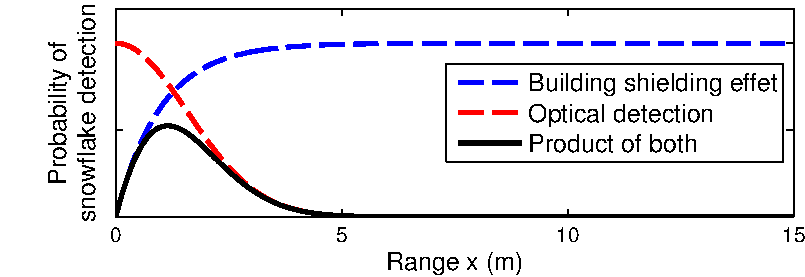
\includegraphics[trim={0.6cm 0 0 0},clip,width=0.7\linewidth]{./img/chap_lidar/ShieldingModel.pdf}
    \caption[Cartoon representation of the interaction between the probability of detecting a snowflake and the diminution of snowflakes due to the shielding effect of the building.]{Cartoon representation of the interaction between the probability of detecting a snowflake (in red) and the diminution of snowflakes due to the shielding effect of the building (in blue). The black line is the product of the two, and bear a close resemblance to the actual histograms extracted from our dataset.}
    \label{fig:CartoonModel}
\end{figure}


\subsection{Sensor Results}
As can be seen from the histograms in Figure~\ref{fig:Histograms}, most sensors exhibit the log-normal or sum-of-log-normal distributions discussed above. We note that for certain days, the distributions are shifted to the right (greater range $x$). In particular, for the 03-21 and the 03-30 distributions, this shift is substantial (on the order of \SI{1}{\meter}). We suspect that for these days, the snowflakes were significantly larger, thus allowing for a stronger optical echo and extended range of detection.

For all sensors, we can also conclude that beyond the range $x>\SI{10}{\meter}$, snowflakes are no longer detected, i.e. they become invisible. A small notable exception would be for the Velodyne, for which snowflakes were detected all the way to $x=\SI{14}{\meter}$, albeit at a significantly reduced rate. Again, we do not think that this would significantly impair their use in conditions similar to our test setup.

\begin{figure}
    \centering
    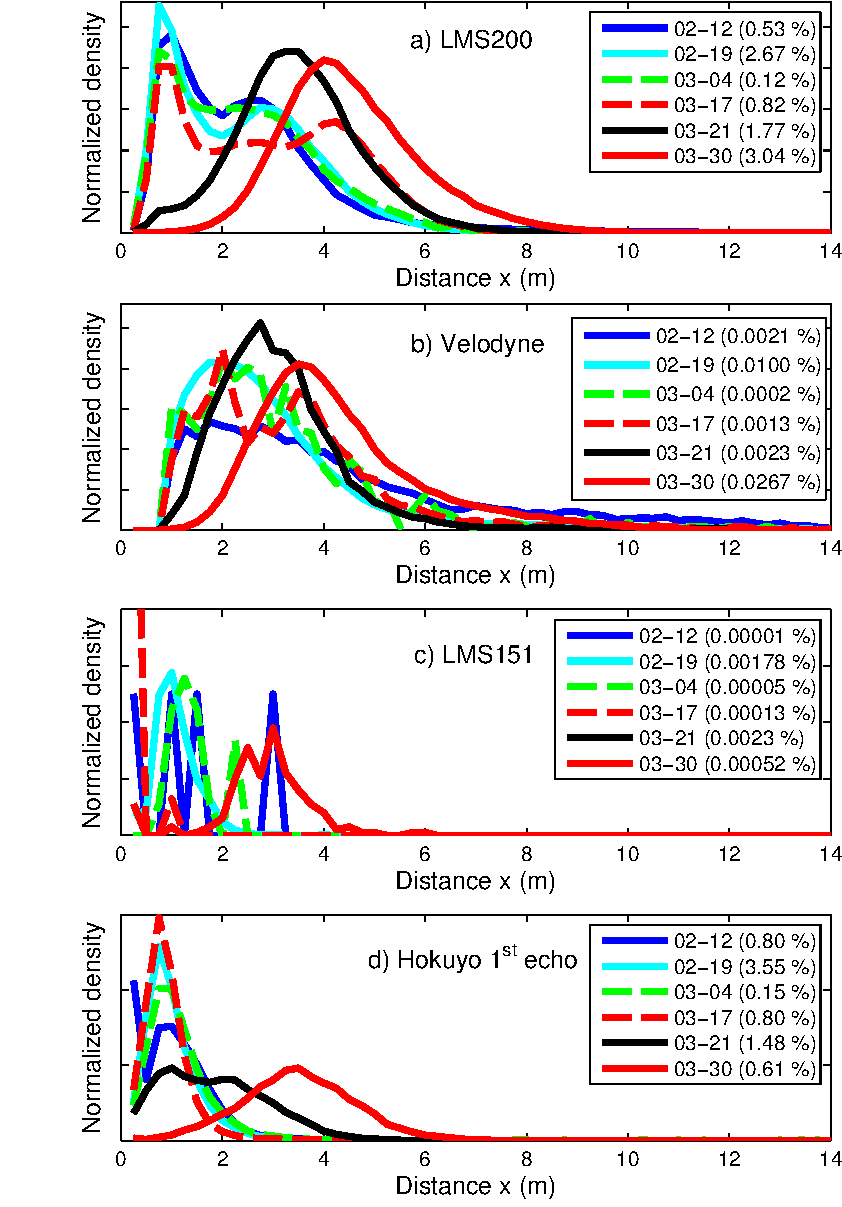
\includegraphics[trim={1.1cm 0 0 0},clip,width=0.80\linewidth]{./img/chap_lidar/Histogram.pdf}
    \caption[Histograms of echoes in falling snow during important snowfall days, as a function of distance reported by the sensor.]{Histograms of echoes in falling snow during important snowfall days, as a function of distance $x$ reported by the sensor. Each histogram has been normalized by its area, for ease of comparison. The numbers in brackets are the fraction of data points in the complete dataset that correspond to snowflake echoes. Note that for the 03-21 dataset, the LMS151 was not working properly: thus no data is included for that day.}
    \label{fig:Histograms}
\end{figure}

\FloatBarrier

\section{Discussion and Conclusion}
\label{sec:chap_lidar_conclu}

\todo{Might be adjusted a bit better to fit the whole document}
In this chapter, we explored the impact of falling snow on the usability of 4 commonly deployed LiDARs. To this end, we collected data during 6 snowstorms in the winter of 2015. Upon analysis, we found that the SICK LMS200 was the most sensitive LiDAR, having a peak average rate of up to 15~\% of echoes coming from falling snow. Meanwhile, all 3 others never exceeded 1~\%. We also presented a simple probabilistic model to take into account the effect of the range on snowflakes interference. Based on a histogram analysis, we concluded that for our experimental setup, this model can be approximated by a log-normal distribution. Most importantly, our data indicate that the impact of snowflakes on LiDAR beyond a range of \SI{10}{\meter} is very limited. 

However, a number of questions remains to explore. For example, as the LiDAR beam travels through the falling snow, its intensity will diminish. Since the maximum range of a LiDAR is heavily related to this beam intensity, we expect the maximum range to be affected during snowstorms. In our setup, we have not witnessed this issue, indicating that this effect probably happens beyond our maximum distance of \SI{20}{\meter}. Another aspect to be investigated is the relationship between the returned intensities and the surface type (ground or snowflakes). Also, because of the shielding effect of the building, very few snowflakes were present at close range; It might be the case that at closer range, a snowflake might be detected at more than one angle, effectively occluding small targets. Moreover, we have not investigated the impact on the measurement noise for the snowy ground surface in the presence of falling snow.


\chapter{\chaptraversabilitytitle}

\section{Introduction (traversability)}
\label{sec:definition}
\begin{itemize}
    \item What is traversability (there is definition problem)
    \item Measure (qualitative and quantitative)
    \item Classification
\end{itemize}

\section{Machine Learning Basics}
\label{sec:machine_learning}

\section{Experimental setup}
\label{sec:setup}
Describe the Husky


\chapter{\chapslamtitle}

\chapter*{Introduction}         % ne pas numéroter
\phantomsection\addcontentsline{toc}{chapter}{Introduction} % inclure dans TdM

Une thèse ou un mémoire devrait normalement débuter par une
introduction. Celle-ci est traitée comme un chapitre normal, sauf
qu'elle n'est pas numérotée.

\section{Data Acquisition}
\label{sec:chap_slam_data_acquisition}

In the following section, we first describe the robotic platform and sensors used to gather our place recognition dataset. We then describe in more details the dataset acquisition procedure and the resulting data.


\subsection{Robotic Platform}
\label{ssec:chap_slam_platform}

The Husky A200 is a medium size (\SI{990 x 670 x 390}{\milli\meter}) \gls*{ugv} developed by \cite{ClearpathWeb}. It is a rugged robot designed for all terrain conditions, therefore well suited for our experiments in the forest. It uses a differential-drive skid steer allowing easy control and in place turns for our data acquisition. It has a maximum speed of \SI{1}{\meter\per\second}, but we generally acquire data at a lower speed to minimize odometry and range data errors. This platform, with a maximum payload capability of \SI{75}{\kilo\gram}, can easily carry all sensors used for our experiments. Our platform is shown in Figure~\ref{fig:chap_slam_husky}. More details about the available devices are presented in Table~\ref{tab:husky_devices}.

\begin{figure}[H]
    \centering
    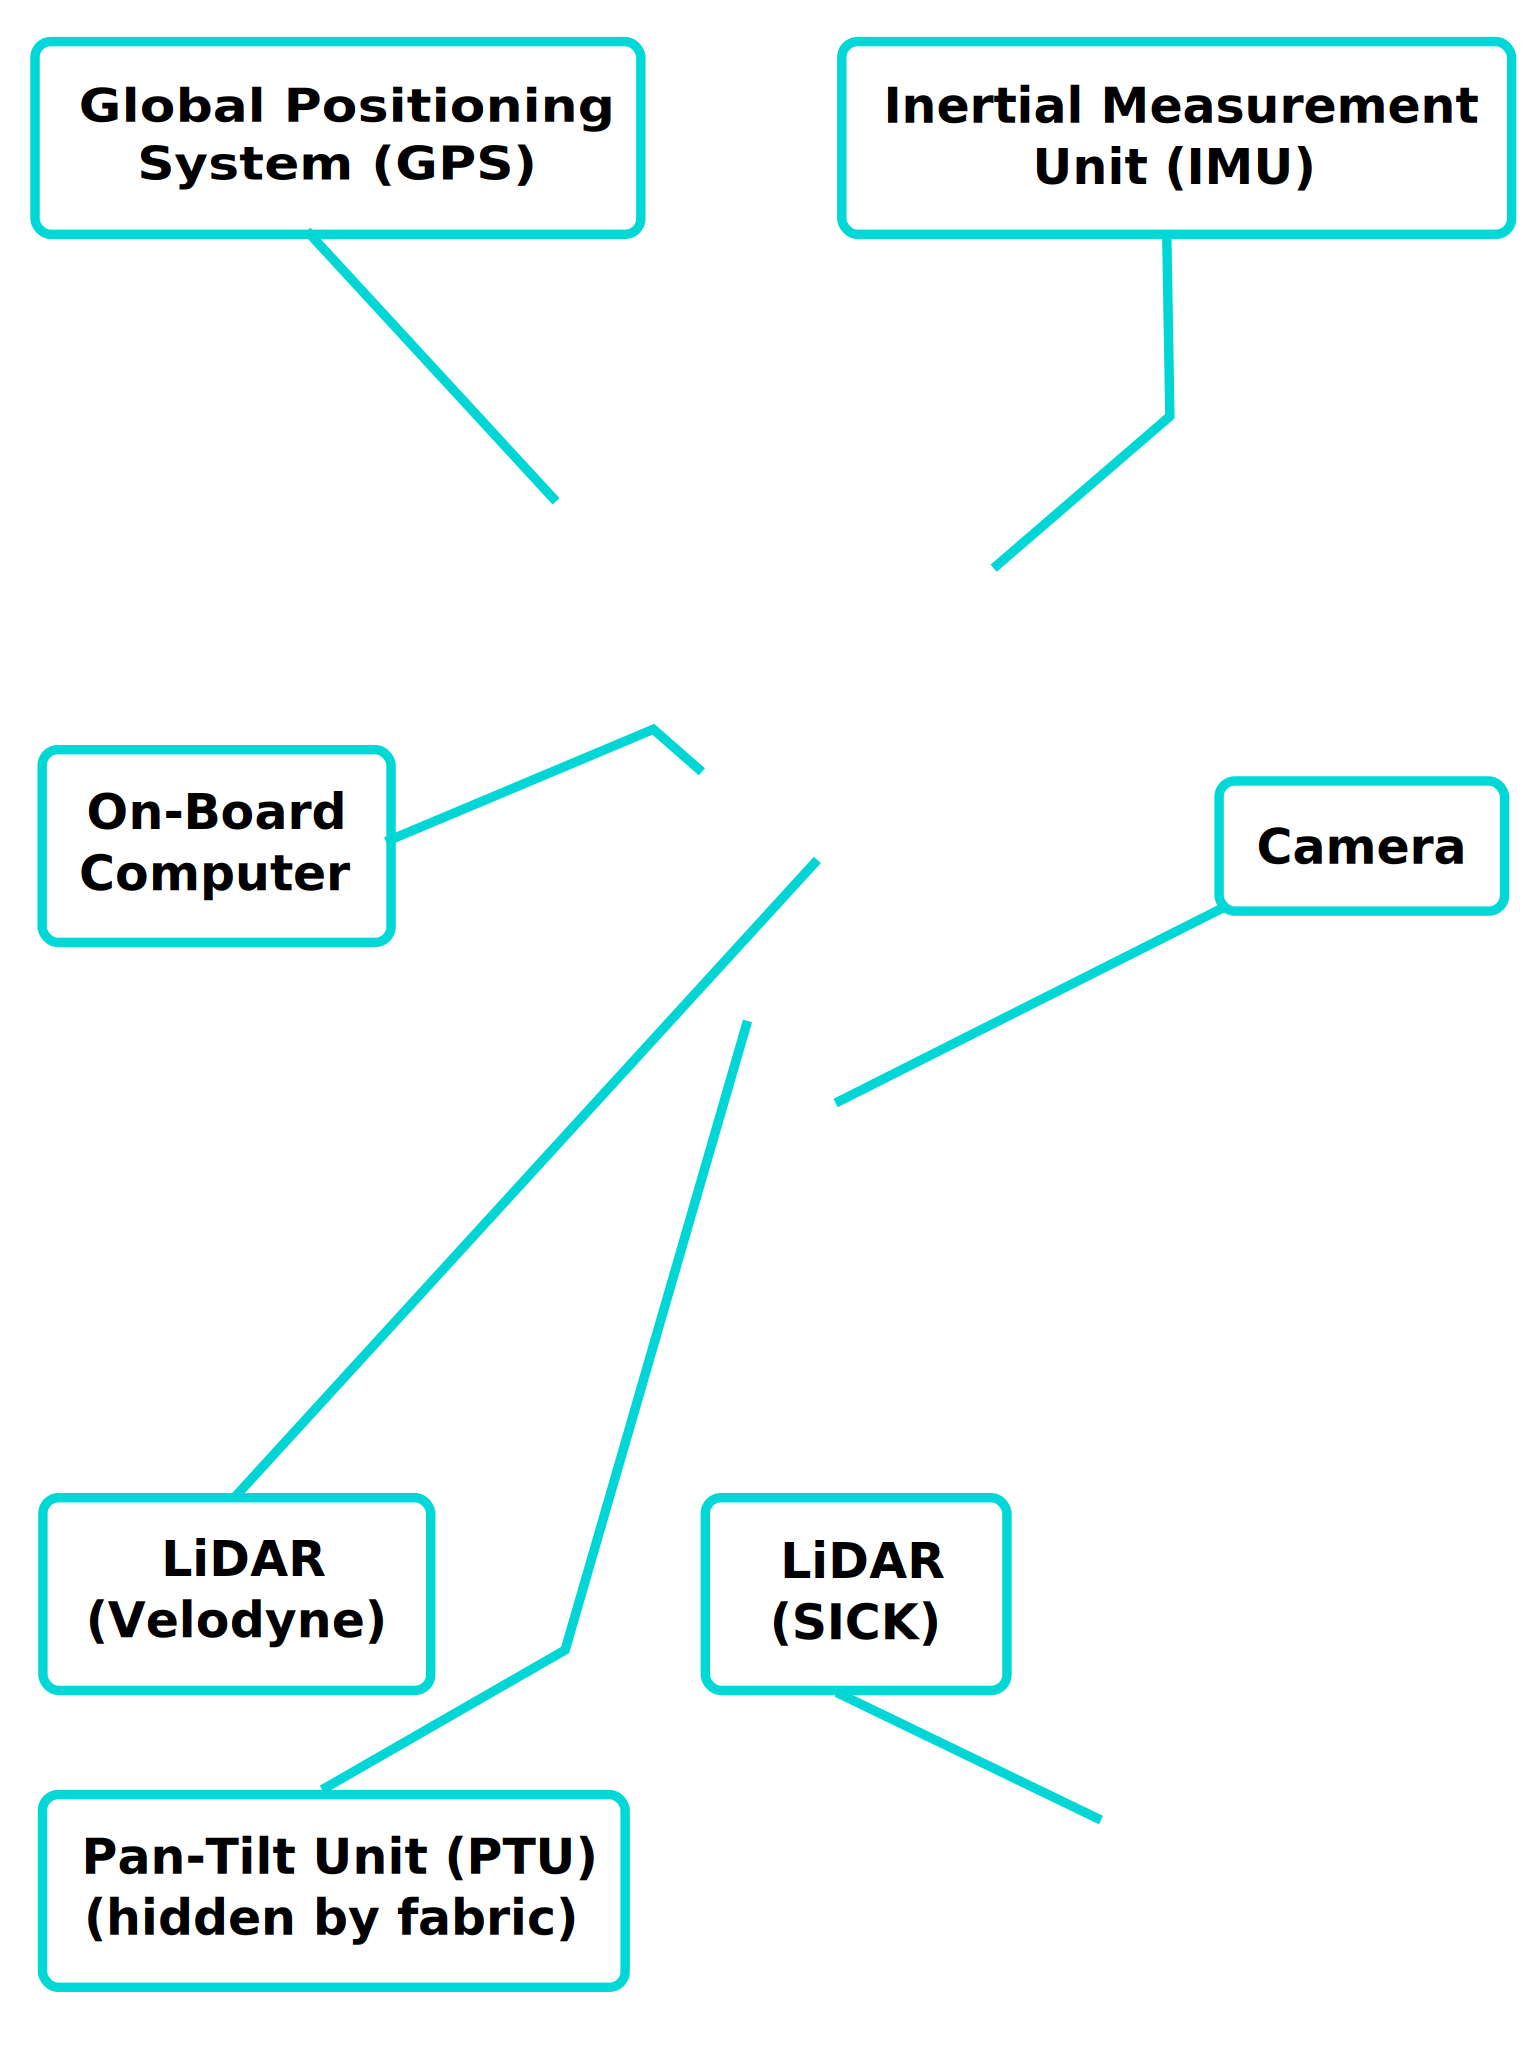
\includegraphics[width=0.98\linewidth]{img/chap_slam/husky_labelled.png}
    \caption{The robotic platform (Husky A200) and the devices used for data acquisition. The SICK \gls*{lidar} is not mounted, but is shown on the bottom right corner of the figure. Note that the \gls*{ptu} is hidden by a cover and the on-board computer is mostly occluded by the Velodyne \gls*{lidar}.}
    \label{fig:chap_slam_husky}
\end{figure}

\begin{table}[H]
    \centering
    \begin{tabular}{@{}llll@{}}
        \toprule
        \textbf{Device} & \textbf{Manufacturer}       & \textbf{Model}  & \textbf{Use}                          \\ \hline
        Computer        & --                          & --              & Data acquisition/synchronisation      \\
        Gateway         & Microhard System Inc.       & VIP2400         & Network and Wi-Fi communication       \\
        Gamepad         & Logitech                    & F710            & Remote control of the robot movements \\
        \gls*{lidar}    & Velodyne                    & HDL-32E         & Point cloud acquisition               \\
        \gls*{lidar}    & SICK                        & LMS151          & Point cloud acquisition               \\
        \gls*{ptu}      & FLIR Motion Control Systems & D46-17          & Rotate the SICK \gls*{lidar}          \\
        \gls*{imu}      & ChRobotics                  & UM6             & Odometry                              \\
        Camera          & Axis                        & M1013           & Visual reference                      \\
        \gls*{gps}      & NovAtel                     & SMART6          & Not used                              \\
        \bottomrule
    \end{tabular}
    \caption{List of devices available on the Husky A200 and their use in our experiments. Note that both \gls*{lidar}s were never mounted at the same time.}
    \label{tab:husky_devices}
\end{table}

The on-board computer (2.4 GHz Intel i5-520M) is an essential element of our experiments, as it connects all devices, acts as a control interface for the robot and stores the acquired data. The computer does not provide a \gls*{gui}, but it is connected to the gateway that broadcasts a WiFi network, allowing \gls*{ssh} communication. The platform is also equipped with a wireless gamepad, which enables manual control of the movements of the robot. Point clouds acquisition is possible using either the SICK LMS151 or the Velodyne HDL-32E. The selected sensor is mounted on the \gls*{ptu}, which remains fixed for the Velodyne, but is rotated with the SICK to merge multiple \gls*{2d} scans into a single \gls*{3d} point cloud. Section~\ref{ssec:chap_slam_platform} gives more details about the resulting point clouds for each sensor.

The sensors described above are essential for our place recognition research, but we also use the wheel encoder along with the \gls*{imu} for odometry estimation and the camera for visual reference of the dataset. Note that we do not use the \gls*{gps}, as we do not want to depend on it for the task of place recognition.


\subsection{Dataset Description}
\label{ssec:chap_slam_platform}

Data acquisition was performed using \gls*{ros}, a set of software libraries and tools created to simplify the development of robotics applications. It provides all drivers for the Husky and our sensors out of the box. Its data publishing system provides timestamps that allows easy synchronization between sensors. The recording tool (rosbag) was used to create our datasets, with data processing performed \textit{a posteriori}.

We produced datasets in two different areas of the Laval University campus. An aerial overview of the path followed by the robot at these two locations is presented in Figure~\ref{fig:chap_slam_path}.

The first site was chosen for its more structured nature and is located between the Alexandre-Vachon and the Adrien-Pouliot buildings. This environment is mostly open, the terrain is smooth and flat and the site contains man-made objects such as buildings, stairs or tables. Examples of pictures acquired by the robot on this site are presented in Figure~\ref{fig:slam_view_building1} and~\ref{fig:slam_view_building2}. This dataset closely resembles the kind of data on which several place recognition algorithms are typically tested on (e.g Freiburg Campus 360 degree 3D scans~\citep{FreiburgDataset}, Robotic 3D Scan Repository~\citep{Datasets}). We will use this data to validate our method.

The second site, chosen for its unstructured nature, is located in a wooded area, also on the Laval University campus. The dataset path starts on a pedestrian walkway, but after its second turn (of approximately \SI{330}{\degree}), it continues for around \SI{100}{\meter} in rougher terrain. This forested environment presents multiple small structures and a lot of occlusions. Figure~\ref{fig:slam_view_forest1} and Figure~\ref{fig:slam_view_forest2} show pictures from the robot camera at this location. This dataset will allow us to better understand the influence of a less structured environment on the place recognition algorithm. In particular, the absence of large flat surfaces and corners typical of buildings, as well as the closeness of the space, will be challenging for place recognition algorithms.

\begin{figure}[H]
    \centering
    \subfloat[]{\label{fig:path_overview}}{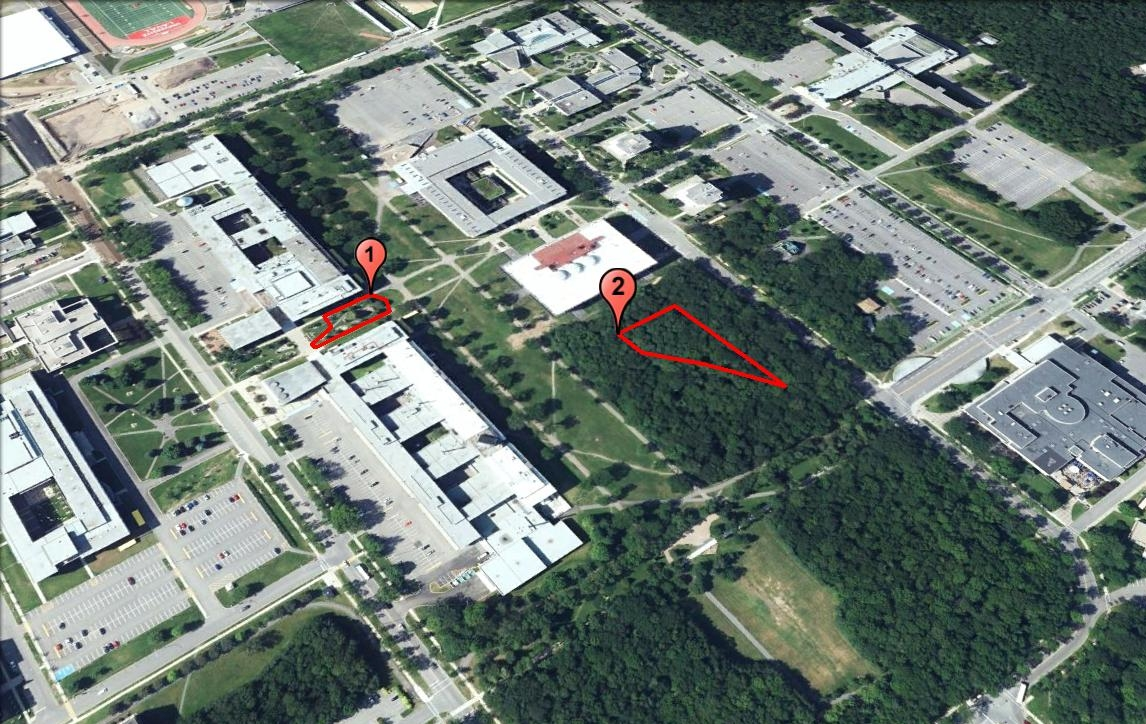
\includegraphics[width=0.995\linewidth]{img/chap_slam/paths.jpg}}\\ \vspace{3mm}
    \subfloat[]{\label{fig:path_building}}{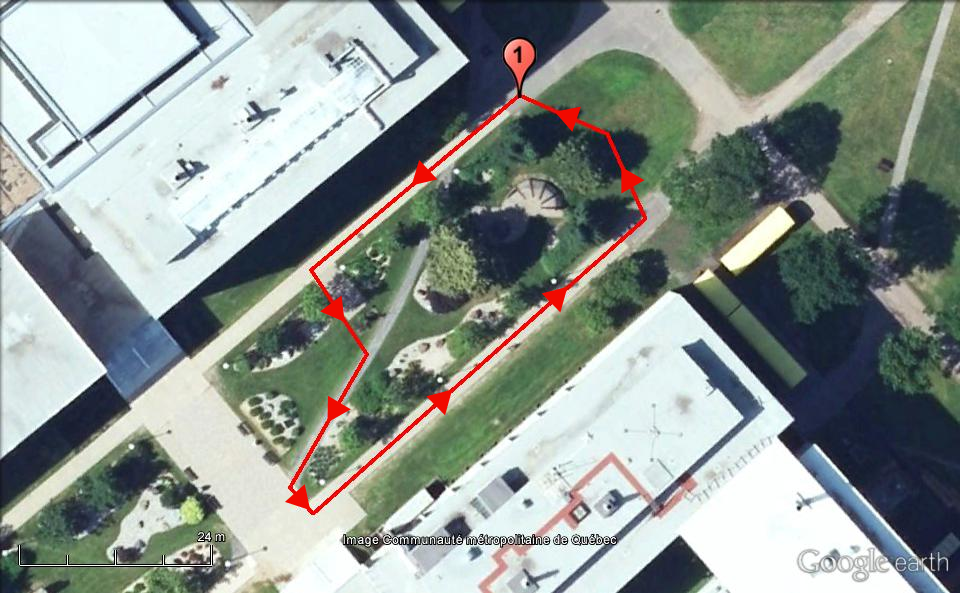
\includegraphics[width=0.485\linewidth]{img/chap_slam/path_building_arrow.png}} \hspace{2mm}
    \subfloat[]{\label{fig:path_forest}}{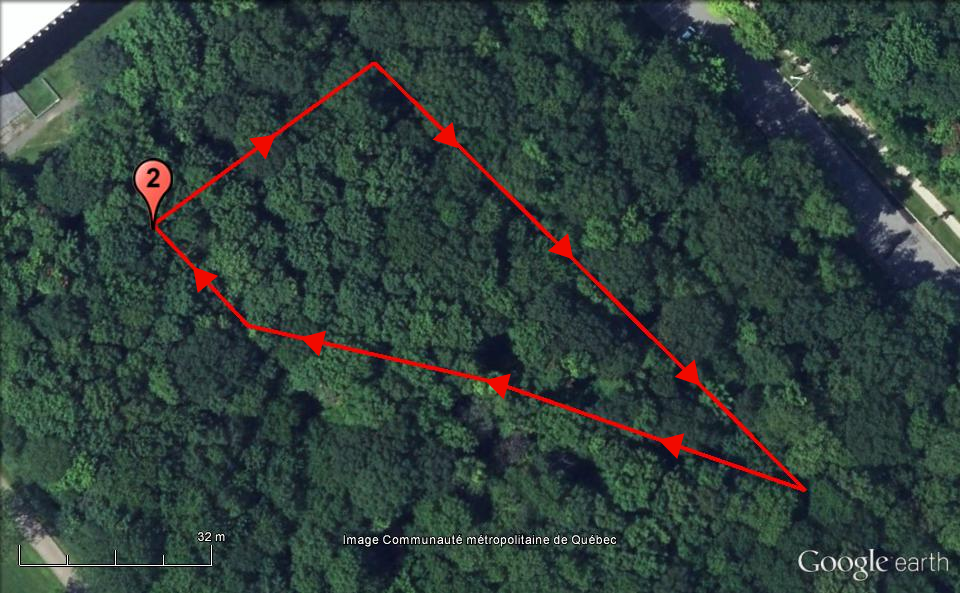
\includegraphics[width=0.485\linewidth]{img/chap_slam/path_forest_arrow.png}}
    \caption{\protect\subref{fig:path_overview} Partial aerial view of the Laval University campus including the two approximate paths followed by the robot for data acquisition. \protect\subref{fig:path_building} Zoomed view of the path followed (counterclockwise from tag 1) in a structured environment. The length of this path is approximately \SI{160}{\meter}. \protect\subref{fig:path_forest} Zoomed view of the path followed (clockwise from tag 2) to create the forest dataset. The length of this path is approximately \SI{275}{\meter}. Images source: Google Earth, (2015)}
    \label{fig:chap_slam_path}
\end{figure}

\begin{figure}[H]
    \centering
    \subfloat[]{\label{fig:slam_view_building1}}{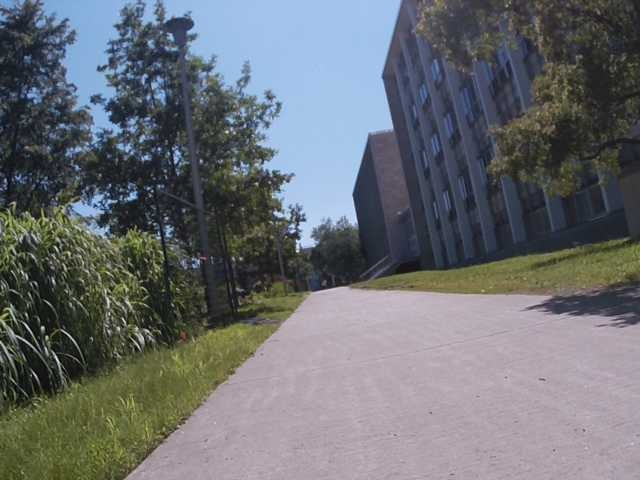
\includegraphics[width=0.47\linewidth]{img/chap_slam/building_view1.jpg}} \hspace{2mm}
    \subfloat[]{\label{fig:slam_view_building2}}{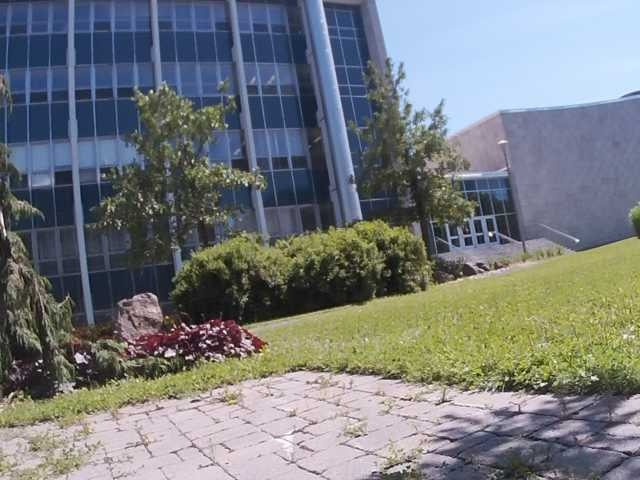
\includegraphics[width=0.47\linewidth]{img/chap_slam/building_view2.jpg}}
    \subfloat[]{\label{fig:slam_view_forest1}}{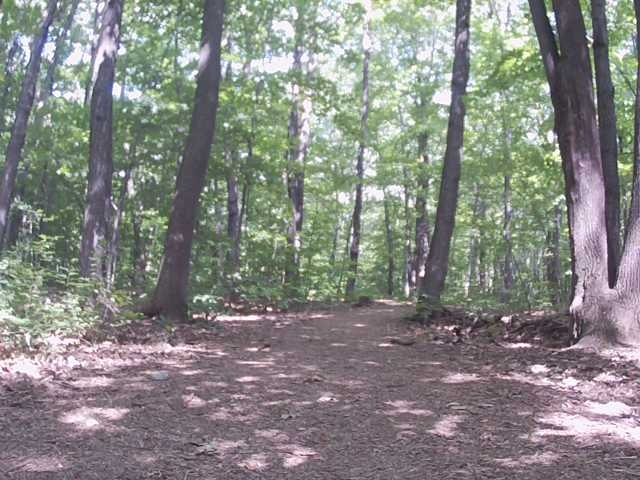
\includegraphics[width=0.47\linewidth]{img/chap_slam/forest_view1.jpg}} \hspace{2mm}
    \subfloat[]{\label{fig:slam_view_forest2}}{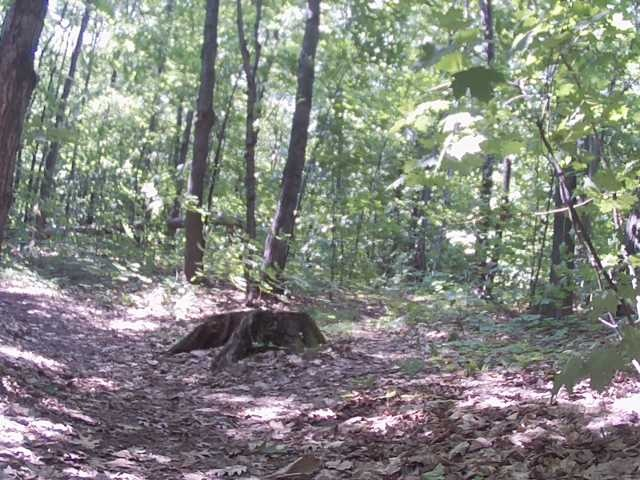
\includegraphics[width=0.47\linewidth]{img/chap_slam/forest_view2.jpg}}
    \caption{Images from the \gls*{ugv} camera during the acquisition of the structured dataset \protect\subref{fig:slam_view_building1} \protect\subref{fig:slam_view_building2} and the unstructured dataset \protect\subref{fig:slam_view_forest1} \protect\subref{fig:slam_view_forest2}.}
    \label{fig:slam_views}
\end{figure}

Besides the influence of the type of environment, we are also interested in the impact of the sensor used and data associated with it. For this analysis, we used two sensors, namely the SICK and the Velodyne, for which you can find details in Table~\ref{tab:slam_sensor_resolution}.

The SICK is a \gls*{2d} \gls*{lidar} with a scanning angle of \SI{270}{\degree}, a resolution of \SI{0.5}{\degree} and an acquisition frequency of \SI{50}{\hertz}. This sensor was placed on the \gls*{ptu} so that the dead angle faced downward. During acquisition, it was rotated around the vertical axis (pan) at a speed of \SI{14.32}{\degree\per\second} for half a turn, while the vehicle was stationary. This procedure allowed the acquisition of 628 \gls*{2d} scans of \SI{540}{\points}, later merged into a single \gls*{3d} point cloud.

The Velodyne, for its part, directly allows \gls*{3d} point cloud acquisition by spinning 32 lasers around its vertical axis. These lasers are evenly distributed between \SI{-30.67}{\degree} and \SI{10.67}{\degree} relative to the horizontal plane. According to the Velodyne datasheet (\cite{VelodyneDatasheet}), the device acquires approximately \SI{700000}{\points\per\second} and publishes at \SI{10}{\hertz}, therefore creating point clouds of \SI{70000}{\points}. Note that these point counts are variable as the rotation speed can change slightly and the use of the \gls*{udp} can lead to some loss of points.

Table~\ref{tab:slam_sensor_resolution} summarizes information about the sensors resolution and \gls*{fov} while Table~\ref{tab:slam_datasets} details the acquisition date and \gls*{lidar} sensor used for each of our datasets.

\begin{table}[H]
    \centering
    \begin{tabular}{@{}lrrrrr@{}}
        \toprule
    \makecell[lc]{\textbf{Sensor}}& \makecell[cc]{\textbf{Horizontal}\\\textbf{resolution}} & \makecell[cc]{\textbf{Vertical}\\\textbf{resolution}} & \makecell[cc]{\textbf{Minimum}\\\textbf{angle}} & \makecell[cc]{\textbf{Maximum}\\\textbf{angle}} & \makecell[cc]{\textbf{Point}\\\textbf{counts}} \\
        \hline
        SICK LMS151      & \SI{0.57}{\degree} & \SI{0.5}{\degree}  & \SI{-45.00}{\degree}  & \SI{90.00}{\degree}  & 339120 \\
        Velodyne HDL-32E & \SI{0.16}{\degree} & \SI{1.33}{\degree} & \SI{-30.68}{\degree}  & \SI{10.67}{\degree}  & 72000  \\
        \bottomrule
    \end{tabular}
    \caption{Details about the point clouds created with our two \gls*{lidar}s. The minimum and maximum angles are given relative to an horizontal plane in the sensor frame of reference and both sensors report \SI{360}{\degree} around the vertical axis. The point counts represent the maximum number of points in the resulting point cloud.}
    \label{tab:slam_sensor_resolution}
\end{table}

\begin{table}[H]
    \centering
    \begin{tabular}{@{}lll@{}}
        \toprule
        \textbf{Site}  & \textbf{Sensor}   & \textbf{Date}                     \\
        \hline
        Structured     & SICK LMS151       & July 16\textsuperscript{th}, 2015 \\
        Unstructured   & SICK LMS151       & July 14\textsuperscript{th}, 2015 \\
        Unstructured   & Velodyne HDL-32E  & May 28\textsuperscript{th}, 2015  \\
        \bottomrule
    \end{tabular}
    \caption{Datasets acquired for place recognition analysis.}
    \label{tab:slam_datasets}
\end{table}

Examples of point clouds from our datasets are shown in Figure~\ref{fig:slam_pointclouds}. We observe that the unstructured environment is more congested and objects are closer to the sensor than for the structured environment. In fact, the average distance of points from the sensor in the unstructured environment is \SI{7.61}{\meter} compared to \SI{9.23}{\meter} for the structured environment. There is also more space without obstacle in the sensor range for the structured dataset. The percentage of points return using the SICK is \SI{82.6}{\percent} on average in the forest dataset compared to \SI{40.2}{\percent} in the structured dataset. These point clouds also illustrate the higher vertical resolution and larger \gls*{fov} of the SICK compared to the Velodyne. The influence of these factors will be discussed in Section~\ref{sec:chap_slam_results}.

\begin{figure}[H]
    \centering
    \subfloat[]{\label{fig:slam_pointcloud_building1}}{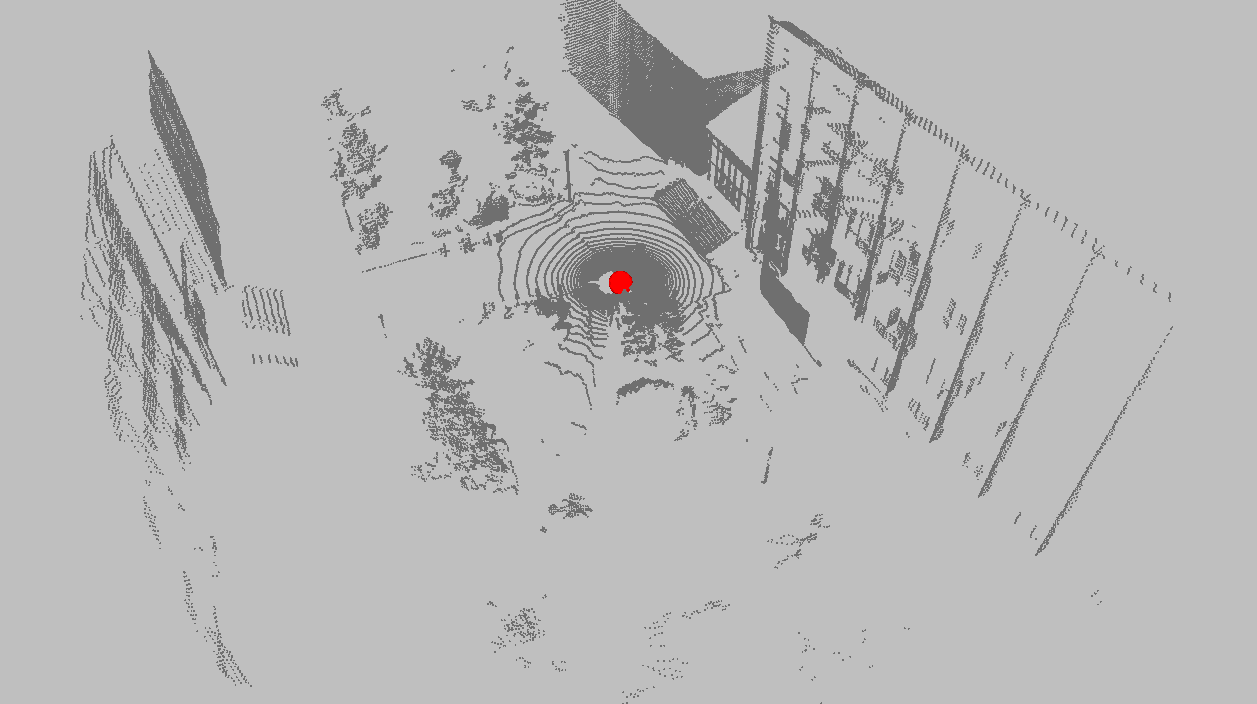
\includegraphics[width=0.47\linewidth]{img/chap_slam/pointcloud_building1.png}} \hspace{2mm}
    \subfloat[]{\label{fig:slam_pointcloud_building2}}{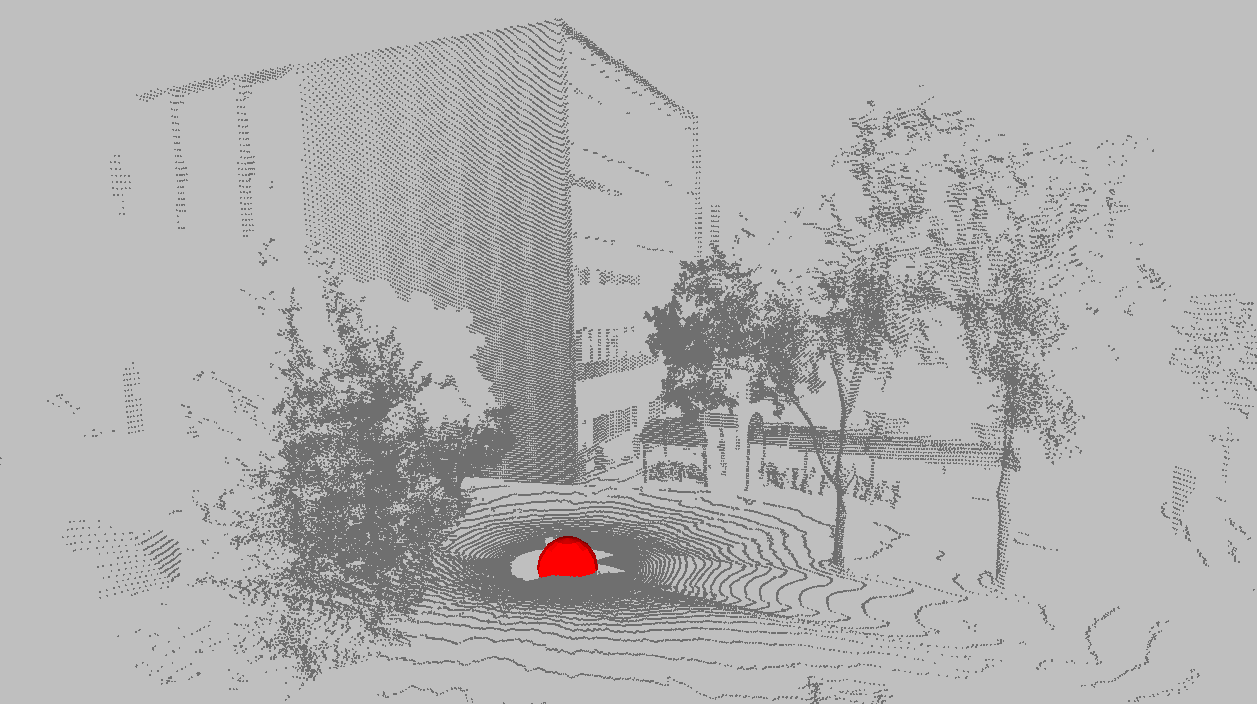
\includegraphics[width=0.47\linewidth]{img/chap_slam/pointcloud_building2.png}}
    \subfloat[]{\label{fig:slam_pointcloud_forest1}}{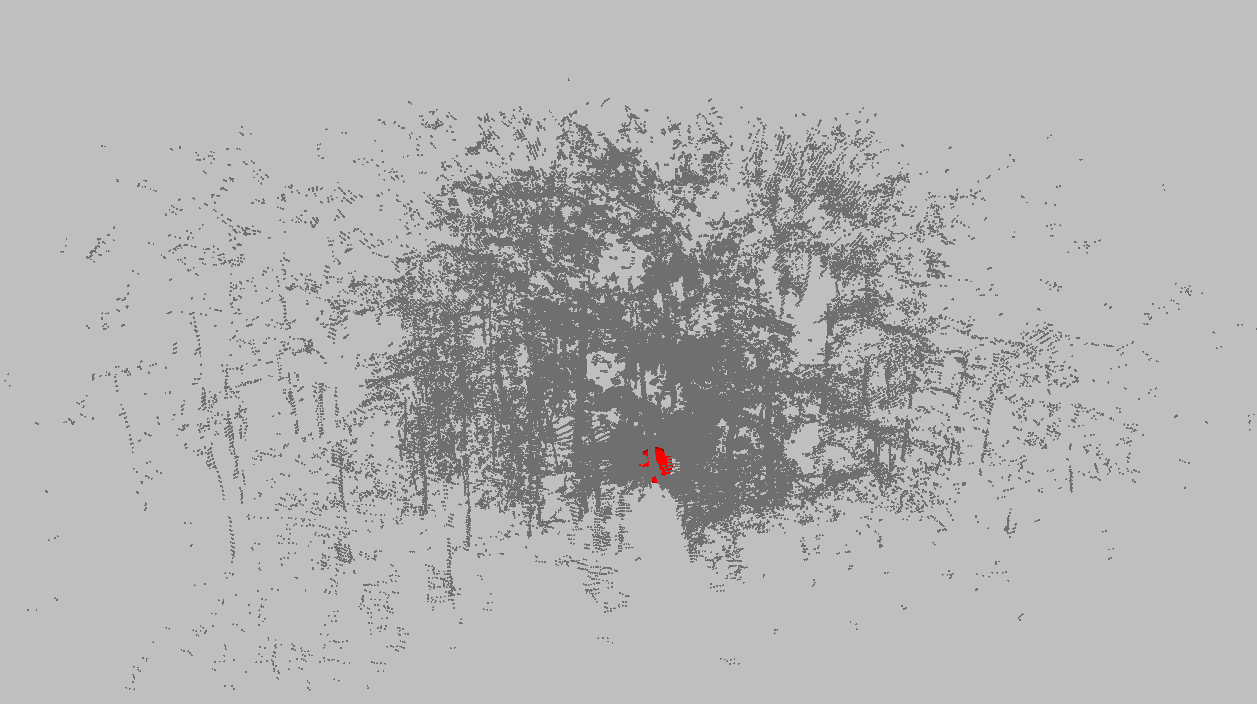
\includegraphics[width=0.47\linewidth]{img/chap_slam/pointcloud_forest1.png}} \hspace{2mm}
    \subfloat[]{\label{fig:slam_pointcloud_forest2}}{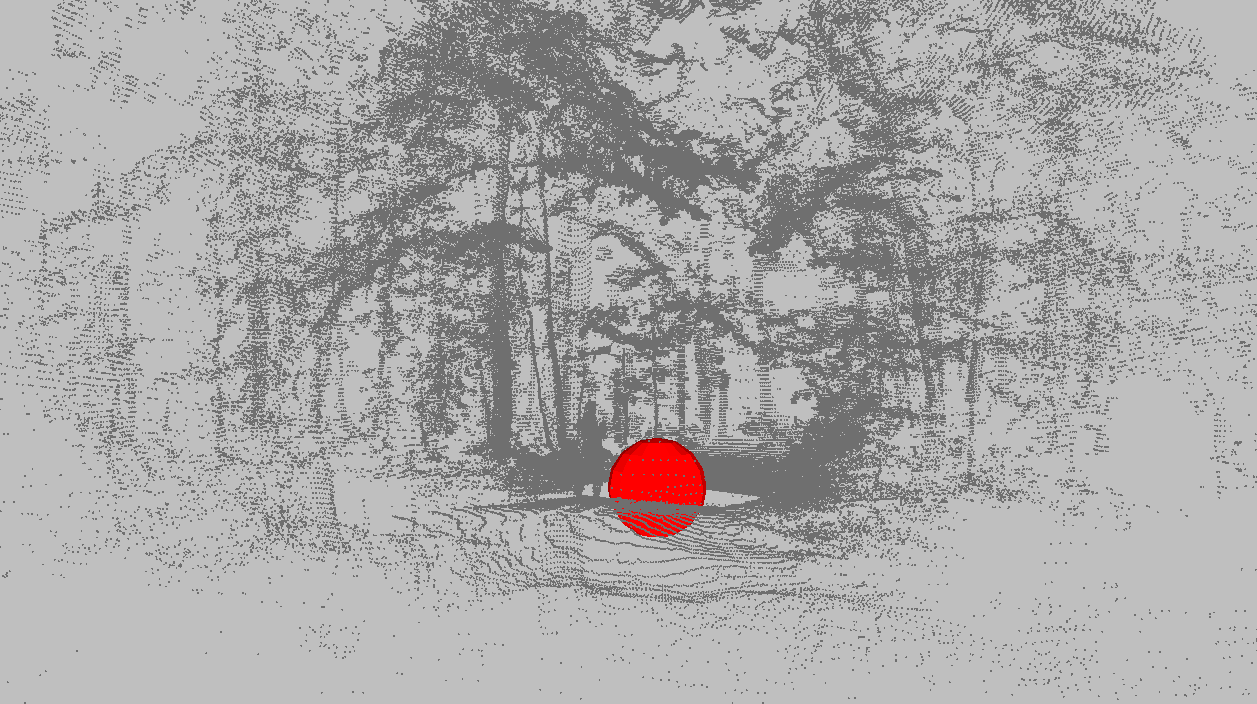
\includegraphics[width=0.47\linewidth]{img/chap_slam/pointcloud_forest2.png}}
    \subfloat[]{\label{fig:slam_pointcloud_velodyne1}}{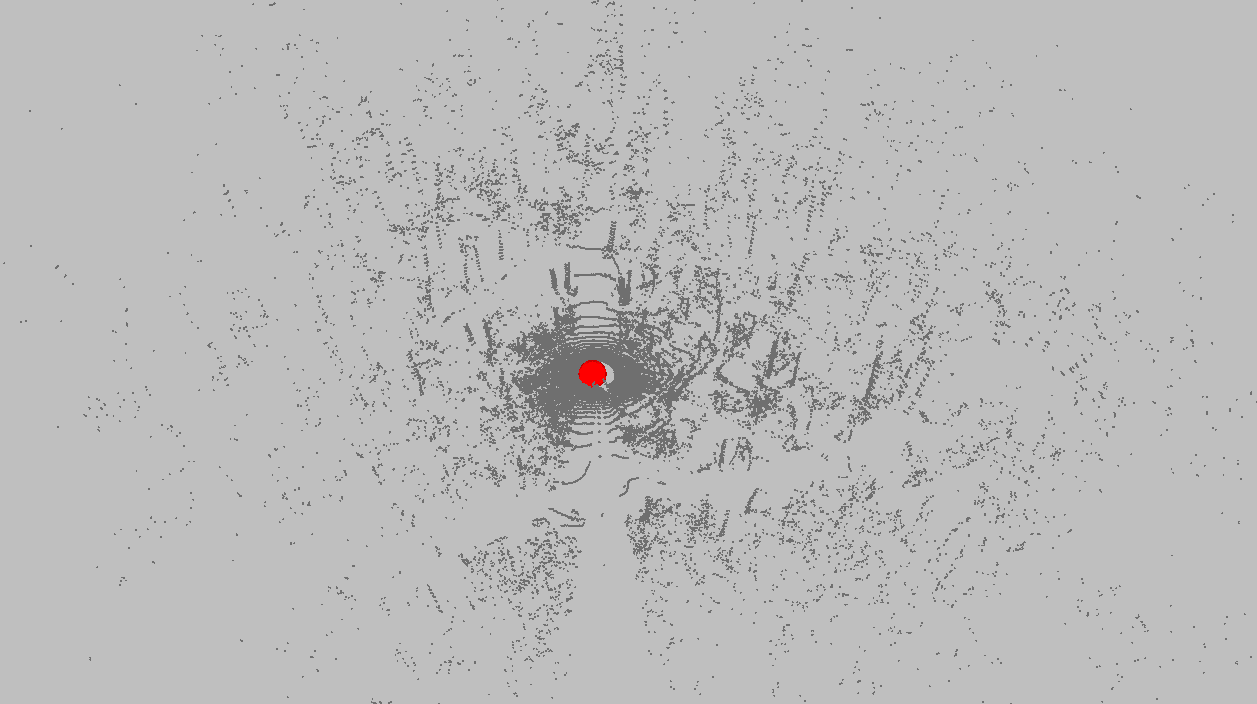
\includegraphics[width=0.47\linewidth]{img/chap_slam/pointcloud_velodyne1.png}} \hspace{2mm}
    \subfloat[]{\label{fig:slam_pointcloud_velodyne2}}{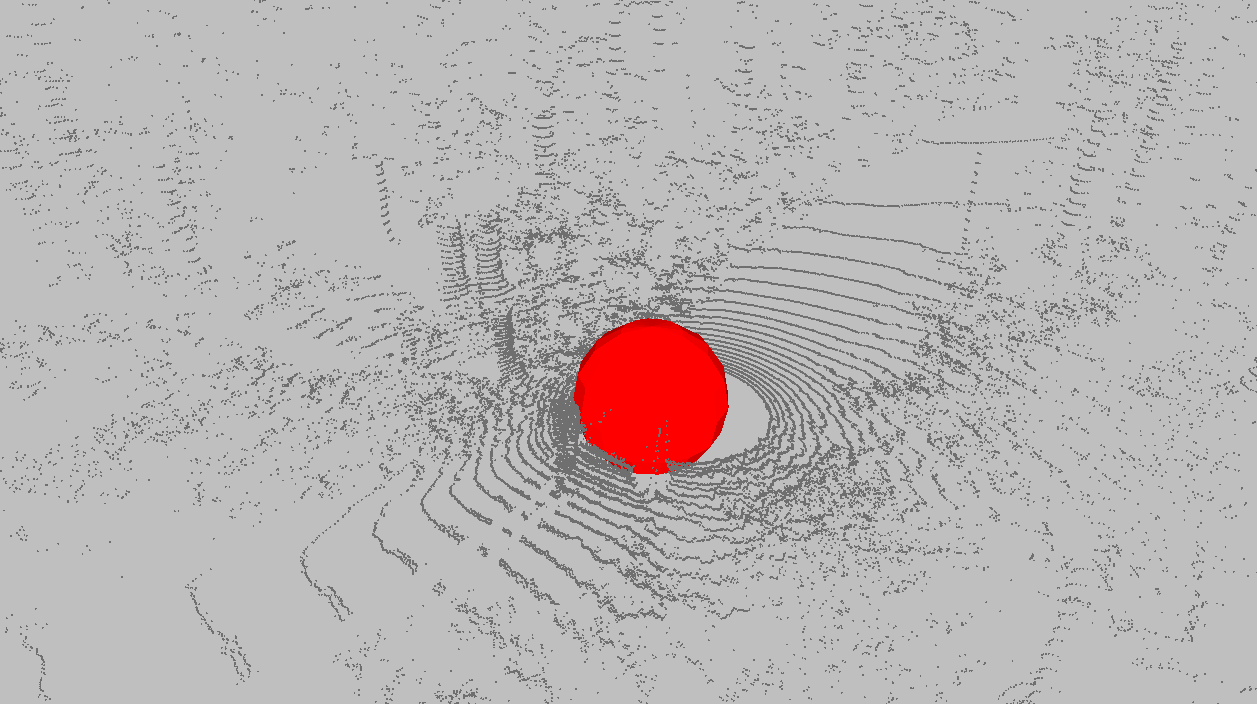
\includegraphics[width=0.47\linewidth]{img/chap_slam/pointcloud_velodyne2.png}}
    \caption{Examples of point clouds from our datasets viewed from different perspectives. \protect\subref{fig:slam_pointcloud_building1} and \protect\subref{fig:slam_pointcloud_building2} show acquisition from the SICK in the structured environment. \protect\subref{fig:slam_pointcloud_forest1} and \protect\subref{fig:slam_pointcloud_forest2} also show point clouds from the SICK, but in the unstructured environment. Finally, \protect\subref{fig:slam_pointcloud_velodyne1} and \protect\subref{fig:slam_pointcloud_velodyne2} show the result of acquisition from the Velodyne in the unstructured environment. Robot position is represented by a red sphere with a \SI{1}{\meter} radius in each picture.}
    \label{fig:slam_pointclouds}
\end{figure}


\section{Place Recognition Algorithm}
\label{sec:chap_slam_algo}

While there are a number of articles presenting place recognition algorithms using different sensors (e.g. camera~\citep{Cummins2011}, stereo-camera~\citep{Cadena2012}), the literature of such algorithms based solely on \gls*{3d} data is limited. For our place recognition analysis, we choose to evaluate on our datasets the state-of-the-art algorithm (at the time of the experiments) developed by~\citet{Steder2011b} on our datasets. We will first describe some fundamental concepts used for place recognition in Section~\ref{ssec:chap_slam_basics} and then we will give an overview of the Steder algorithm itself in Section~\ref{ssec:chap_slam_algo}. For the interested reader, the full details of the algorithm are available in~\citep{Steder2011b}.


\subsection{Fundamental Concepts}
\label{ssec:chap_slam_basics}

The following subsection is an introduction to basic concepts for understanding \gls*{3d} place recognition algorithms in general. In particular, conventional methods for representing and comparing \gls*{3d} acquisitions will be presented.

\subsubsection{Feature Keypoints and Descriptors}
\label{ssub:feature_keypoints_and_descriptors}

The first step in determining whether or not a place has been visited before, is to convert the sensor data into a format that is more convenient for identification. The generally-adopted representation is a vector of real numbers, called descriptor. This mathematical representation aims at being more compact than the original data while trying to capture significant characteristics from a recognition point of view.

A descriptor can be \emph{global}, meaning that it tries to capture information about the whole scan, or \emph{local}, meaning that it does the same but only for a specific subregion of the scan. When using local descriptors, one needs to select the keypoints around which the descriptors will be extracted. These keypoints can be at pre-determined and fixed locations (e.g. division in a simple grid) or selected using more refined algorithms. A common practice for the latter is to choose keypoints in so-called interesting regions which are often defined as regions of high gradient (e.g. edges, corners), as these region generally contains more information than smooth surfaces. Note that, for simplicity, we might use the term \textbf{features} as a more general term for keypoints and their respective descriptors in the remainder of this document.

The concepts of keypoints and descriptors first originated from the computer vision literature. More recently, they have been adapted for \gls*{3d} data. Some popular examples of features for both types of data are shown in Table~\ref{tab:features_examples}. Note that some algorithms propose solutions for both keypoints detection and descriptors (e.g. SIFT, NARF). However it is not mandatory to use them together as any combination is generally valid. While all features are different, they were all developed with the same goals in mind:
\begin{itemize}[label=$\bullet$,noitemsep,topsep=0pt]
    \item Distinctiveness: each feature should be easily differentiable with respect to others.
    \item Repeatability: the feature values should be stable under changes including:
        \begin{itemize}[label=$\circ$,noitemsep,topsep=0pt]
            \item Transformations: rigid transformation for point clouds and projective transformation for images, but also changes in the pose of the objects and/or the viewpoint.
            \item Noise: small variations in measurements (range/intensity) and occasional erroneous values (points/pixels).
            \item Resolution: the number of points or pixels representing a given area.
        \end{itemize}
\end{itemize}


\subsubsection{Range Image and NARF Feature}
\label{ssub:NARF Features and Range Image}

In this subsection, we present the NARF keypoints and descriptors, as well as the \gls*{3d} data representation on which they rely: the range image. We will see that the place recognition algorithm, presented in Section~\ref{ssec:chap_slam_algo}, relies on this \gls*{3d} representation to determine a matching score between scans.

Range images represent a \gls*{3d} data point by a pixel position (i.e x and y) and a range value. Note that the position of the pixel actually represents a horizontal and vertical angular position. For an omnidirectional \gls*{lidar} scan, the corresponding range image is a spherical projection of the points from the center of the sensor. Range images can be better defined by the constraints they must meet to be valid.

Firstly, converting a \gls*{3d} scan into a range image requires the acquisition to originate from a single view point and to have a single range value per pixel. It is therefore not possible to use point clouds acquired with multi-echoes \gls*{lidar}s or produced by merging multiple scans. Fortunately, the latter constraint is met in our datasets.

Secondly, every pixel in a range image must have a value. Since \gls*{lidar}s have a minimal and a maximal range, the data points outside this interval are ignored. Similarly, when a laser beam hits a highly absorbing or a reflecting surface at an angle, the sensor will not get any return. Such missing data points cause pixels of the range image to have no value, the latter are considered as far range (i.e. the maximum range of the sensor).

Finally, the resolution has to be adjusted so that each pixel of the resulting range image covers the same angular resolution vertically and horizontally. Images being discretized in pixels, the values of these can either be a weighted average of the laser beam ranges, or the value of the smaller range within his area, depending on the user preference. The converted scans have a dense and uniform representation similar to grayscale images, allowing the reuse of standard image processing techniques. Examples of range images can be seen in Figure~\ref{fig:chap_slam_range}.

\begin{figure}[H]
    \centering
    \subfloat[]{\label{fig:range_building}}{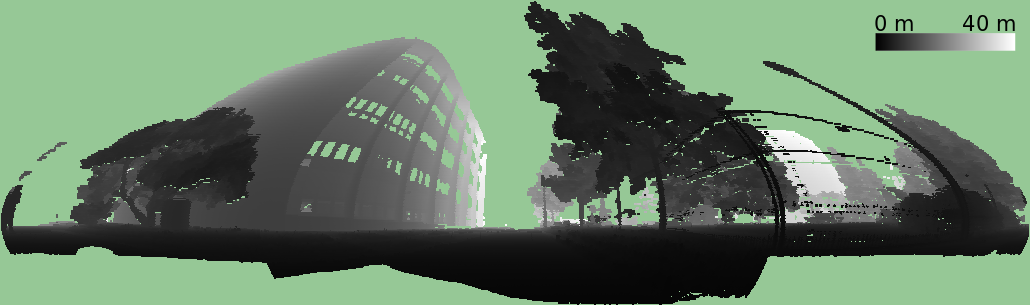
\includegraphics[width=0.995\linewidth]{img/chap_slam/range_building01_scale.png}}\\
    \subfloat[]{\label{fig:range_forest}}{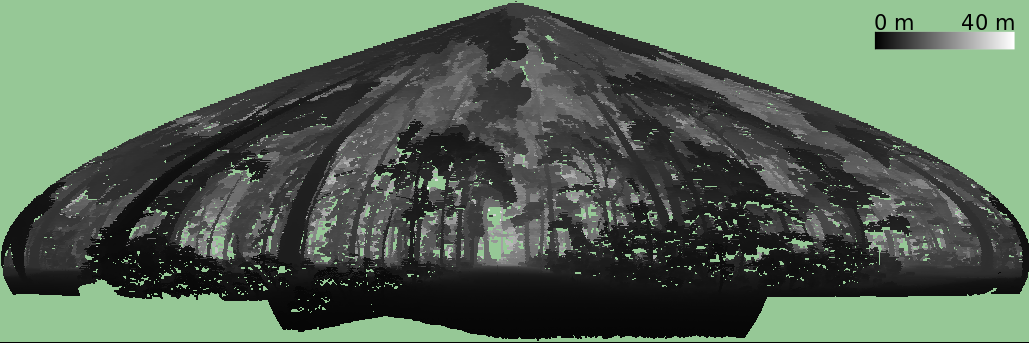
\includegraphics[width=0.995\linewidth]{img/chap_slam/range_forest01_scale.png}}
    \caption[Examples of range images from the two datasets.]{Examples of range images for the Structured-SICK dataset \protect\subref{fig:range_building} and the Unstructured-SICK dataset \protect\subref{fig:range_forest}. Note that objects appear distorted due to the projection on the plane. The background color (light green) corresponds to areas without laser return. All other pixels represent ranges between \SI{0}{\meter} (black) and \SI{40}{\meter} (white).}
    \label{fig:chap_slam_range}
\end{figure}

As indicated previously, feature keypoints are generally chosen in high gradient regions of the \gls*{3d} inputs. A problem arises when the input data is in the form of a point cloud, as it is impossible to distinguish edges caused by object boundaries from those caused by occlusion. Figure~\ref{fig:chap_slam_edges} present an example of a partial range image and the corresponding point cloud, where you can see edges caused by an object boundary and edges caused by the occlusion of this object. Edges caused by occlusions can generate meaningless keypoints and the descriptors built based on these keypoints leads to a poor representation of the environment, which can reduce the place recognition performance. This is particularly useful in our context of complex environments such as forest, because there are significant occlusions. The article describing the NARF features~\citep{Steder2011a} details how using range images allow to differentiate these two types of edges.

\begin{figure}[H]
    \centering
    %\subfloat[]{\label{fig:range_edge}}{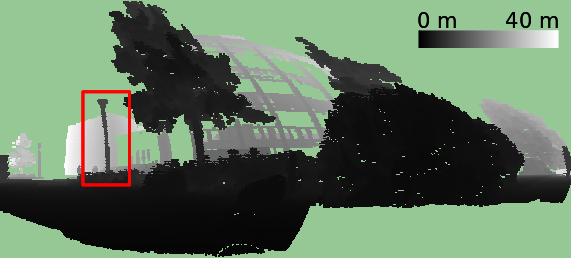
\includegraphics[width=0.507\linewidth]{img/chap_slam/range_building21_adjusted.png}}
    %\subfloat[]{\label{fig:pointcloud_edge}}{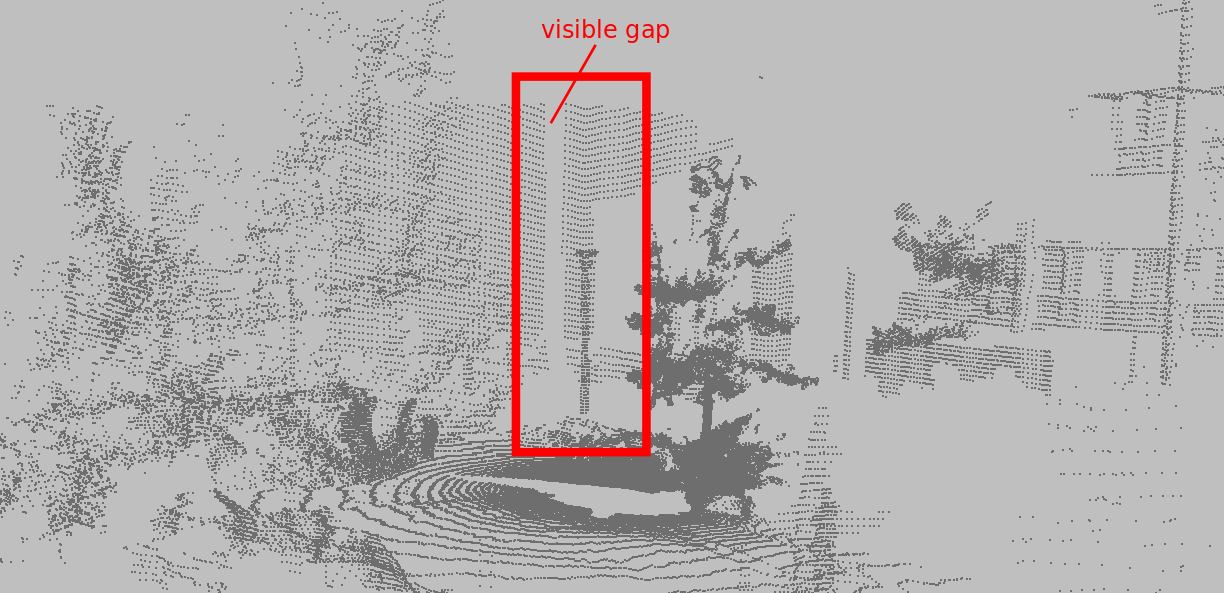
\includegraphics[width=0.473\linewidth]{img/chap_slam/pointcloud_building21.png}}
    \subfloat[]{\label{fig:range_edge}}{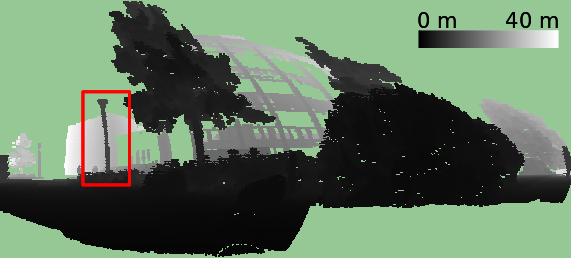
\includegraphics[width=\linewidth]{img/chap_slam/range_building21_adjusted.png}}\\
    \subfloat[]{\label{fig:pointcloud_edge}}{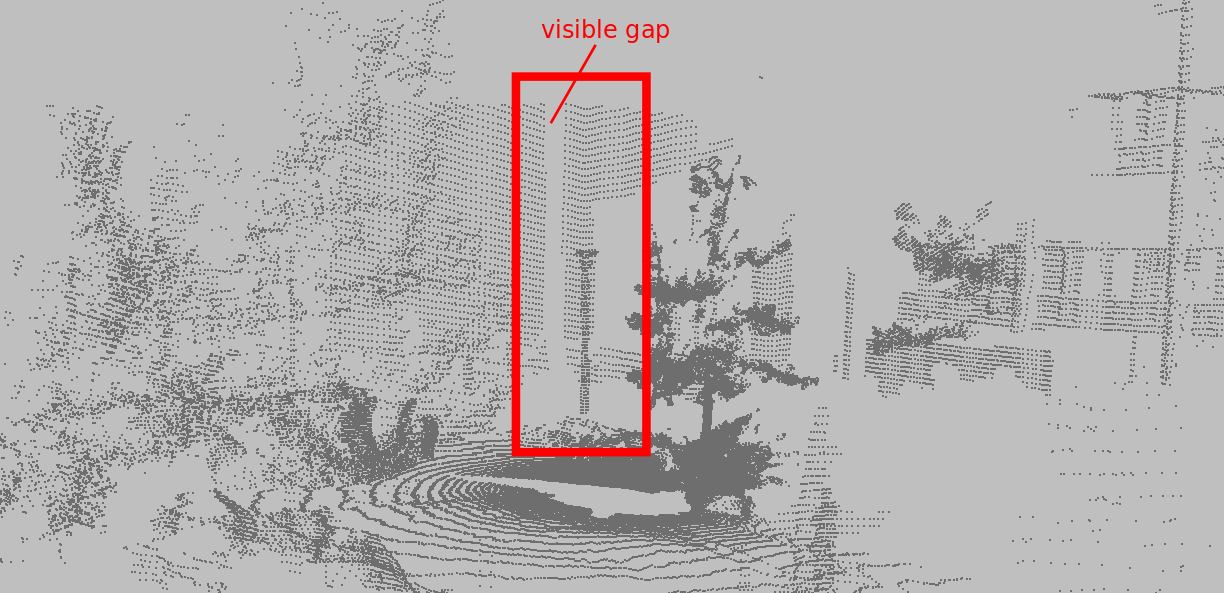
\includegraphics[width=\linewidth]{img/chap_slam/pointcloud_building21.png}}
    \caption[Example of a partial range image and the corresponding point cloud with an example of edge caused by an object border.]{Example of a partial range image \protect\subref{fig:range_edge} and the corresponding point cloud \protect\subref{fig:pointcloud_edge}. The red rectangle highlight a region of the environment where, from the robot point of view, a lamp post partially occludes a building wall. In the point cloud, this configuration leads to edges on both the lamp post boundary and the wall itself. In reality, the information contained in this scan does not allow to know what is behind the post and the edges of the wall are most likely artifacts caused by occlusion. In contrary, the range image is built taking into account the position of the sensor, thus allowing to consider only the boundary of the lamp post as edges and ignoring edges on the wall. Indeed, one can ignore the gap in the wall for the range image, as it is readily explained by the occlusion of the range image. Determining this occlusion is not possible by nature in a point cloud.}
    \label{fig:chap_slam_edges}
\end{figure}

The last item to be discussed concerning the NARF features is the descriptor structure. In order to create this NARF descriptor, one must first compute the normal to the surface at the keypoint location. A star pattern, as shown in Figure~\ref{fig:narf_descriptor}, is then overlay on top of a small range image patch, as seen by an observer looking at the keypoint along the normal. Each beam of the star pattern corresponds to a single value in the final descriptor. This value captures how much the pixels changes under the beam (i.e. its gradient). A unique orientation around the normal is finally determined, to ensure that the NARF descriptor is rotation invariant. This orientation corresponds to that of the beam having the largest value. An interesting characteristic of the NARF descriptors is that each of them encodes its own local coordinate system, allowing for a complete six degrees of freedom pose identification. This is possible due to the fact that we know the normal to the local surface patch and the unique orientation around the latter. Figure~\ref{fig:narf_descriptor} illustrates how descriptors are computed.

\begin{figure}[H]
    \centering
    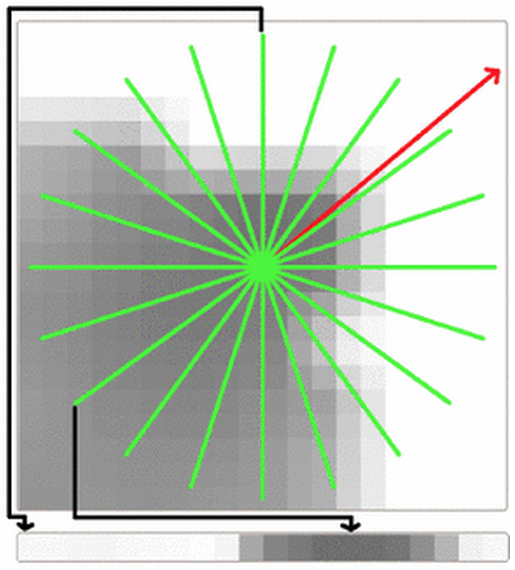
\includegraphics[width=0.4\linewidth]{img/chap_slam/narf.png}
    \caption[Illustration of a NARF descriptor calculated on a range image patch.]{Illustration of a NARF descriptor calculated on a range image patch. Each of the 20 green beams are represented by a single value in the descriptor vector, which is represented at the bottom. In addition, the position in the descriptor of two of those beams are marked with black arrows. The value attributed to a beam represent how pixels change under it. More presicely, beams that lie on a flat surface have low values and beams going over a high gradient (i.e. potential object border) have high values. The red arrow (pointing to the top right) show the extracted dominant orientation around the normal of the patch. From~\cite{Steder2011a}.}
    \label{fig:narf_descriptor}
\end{figure}


\subsubsection{Scans Comparison}
\label{ssub:scans_comparison}

The last item to be discussed in this subsection is the method used to compare two scans. This is usually accomplished using the descriptors representing the scans. Since a descriptor is a vector of values representing the underlying data, two descriptors with very similar corresponding values should also represent similar entities (e.g. objects). Consequently, similarity between descriptors are generally computed using a simple distance metric (e.g. Euclidean distance, cosine distance).

The comparison between two scans using global descriptors is usually computationally inexpensive. Indeed, a single descriptor is computed for each scan and the comparison between two of them simply requires the computation of only one distance metric. Also note that for global descriptors, there is no such thing as keypoints and the geometric information is intrinsically included in the descriptor itself. A major drawback of such comparison approach is the high sensitivity to local changes of the environment, which may for example be caused by dynamic objects. This approach is also sensitive to small changes in position of the sensor of the sensor.

From a computational point of view, scans comparison based on local descriptors are more demanding. Indeed, besides having to calculate several keypoints and their associated descriptors, a method must be chosen to compare two scans over all features. In addition, the geometric relationships between features provides important cues about scans and may thus be considered to improve reliability of place recognition, albeit at a greater processing cost. Fortunately, using local features generally yield more robust results regarding local changes and also provides more comparison flexibility for the user. We will see a number of techniques for comparing scan using local features in the following paragraphs.

A first approach to compare \gls*{3d} scans with local descriptors consists in finding local descriptors correspondences between the scans. These correspondences are use to check if there is a valid transformation that aligns the scans. As we deal with data from real, noisy sensors, the vectors of real numbers representing the features (i.e. the descriptors) will never be exactly the same from one scan to another. A simple solution to this problem is to use the concept of nearest neighbor to identify the correspondences. One has to bear in mind that several descriptors may have no valid match due to background clutter or change in the view point. \cite[Section 7.1]{Lowe2004} describes how to remove most of those false matches by comparing the distance of the closest neighbor to that of the second-closest neighbor. The intuition is that this second best match is an incorrect one and using this ratio, only matches that have the closest neighbor significantly closer than the closest next match will be used, therefore improving reliability.

Once the corresponding descriptors between two scans have been identified, they are used to determine if there is a valid rigid \gls*{3d} transformation that align the underlying keypoints. The existence of such valid transformation serves as a first check on the similarity between two scans. This step also requires a criteria on the number (or ratio) of features correctly aligned, thereby identifying the scans as originating from the same place or not. This is generally achieved using the RANSAC algorithm~\citep{Fischler1981}. This rigid transformation estimation is computationally expensive, but has the advantage of being very discriminative. Additionally, it provides relative pose between scans, which is not possible using global descriptors. The relative pose can, for example, be used to determine odometry or during map creation process. Figure~\ref{fig:chap_slam_features_correspondences} shows keypoints from two scans of our dataset, as well as examples of correspondences.

A second solution, that speed up comparison when searching for potential matches between scans, is to represent the set of features of each scan by a \gls*{bow}~\citep{salton1983mcgill}. The concept of \gls*{bow} was first used for documents classification. In this context, \gls*{bow} represented a document by a vector of occurrence counts of a vocabulary without taking into account their ordering. In our case, the descriptors are made up of real numbers which allows for an infinity of them; therefore they cannot be used directly as words. The solution to this problem is to use a clustering algorithm such as k-means~\citep{MacQueen1967} to create groups that will represent words, a process known as \emph{quantization}. For instance, \citet{Cummins2008} present examples of visual words that typically correspond to the cross-piece of windows and other words that correspond to top-left corner of windows. An advantage of using k-means is that it is an unsupervised algorithm, meaning that no manual labeling effort is required. Because the \gls*{bow} approach avoids having to compare all potential feature correspondences between the scans, it significantly reduces the processing time. On the other hand, this method removes all information regarding the geometric configuration of keypoints in the scans, which might induce unwanted perceptual aliasing~\citep{Mariottini2011}. This is a rather general representation with for which the comparison is relatively fast to compute. Note that the visual dictionary is generally created in advance, in offline manner, using a large collection of local descriptors gathered under similar conditions and for similar scenes.

The chosen place recognition method will depends on several factors such as the available hardware resources, the desired processing time and the required reliability of the results. Using features correspondences along with geometric check is more computationally expensive than using the \gls*{bow} approach, but results are also more reliable. However, we will see in Section~\ref{ssec:chap_slam_algo} that it is possible to take advantage of the combined use of these methods.

\begin{figure}[H]
    \centering
    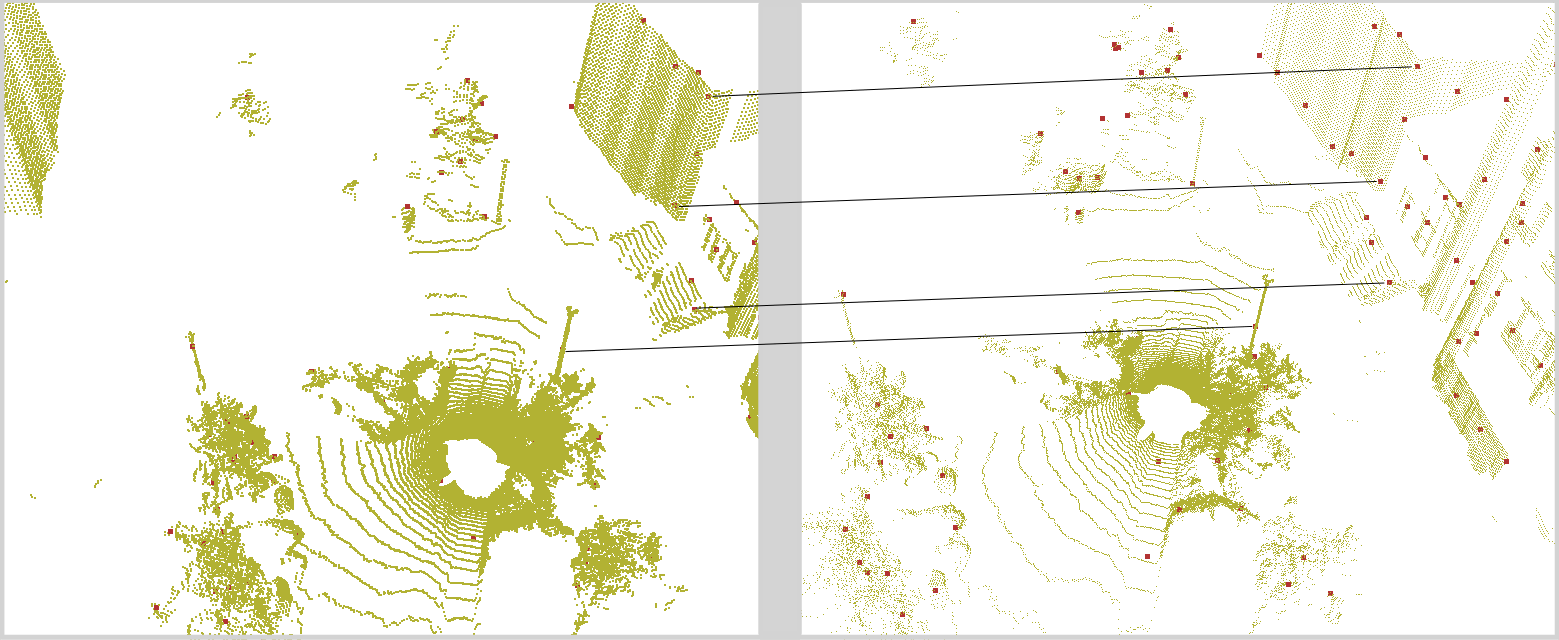
\includegraphics[width=0.995\linewidth]{img/chap_slam/features_line.png}\\
    \caption[Examples of NARF keypoints found for two different scans with examples of correspondences.]{Examples of NARF keypoints (red squares) found for two different scans of the structured dataset. Black lines illustrate examples of valid correspondences found across scans. These NARF keypoints show stability under changes, such as viewpoint, noise and resolution.}
    \label{fig:chap_slam_features_correspondences}
\end{figure}


\subsection{Overview of the Algorithm}
\label{ssec:chap_slam_algo}

In the following section, we will describe the algorithm used for our experiments, but we will first describe the general idea of the technique and the two articles describing it~\citep{Steder2010}~\cite{Steder2011b}. For the place recognition algorithm to be used, one must first acquire a set of 3D scans at approximately regular interval with a robot equipped with an omnidirectional \gls*{lidar}. This initial set of scans for a given environment, dubbed scans database ($D$), act as a representation of all known and visited places. Subsequent scans are used to determine if a match can be found in this database, and thus establish metrics such as precision and recall. Note that this experimental procedure was repeated in different indoor and structured outdoor environments and with different \gls*{lidar}s for both original articles.

In the first version of the algorithm \citep{Steder2010}, they compared a newly acquired scan ($z^*$) against all scans from the database ($z^1,...,z^{|D|}$), only using NARF features correspondences. As mentioned previously, these features encode a full \gls*{3d} pose, which in theory allow the determination of the transformation that align two scans based on a single features correspondence. This meant that there was as many candidate transformations as there was features correspondences between a newly acquired scan ($z^*$) and a single scan ($z^i$) from the database. Using a series of rules, a score was assigned to each of these transformations. This score reflected the system belief that this transformation was an actual match. The transformation having obtained the highest score is used to align $z^*$ with $z^i$.

Although this technique yielded high recognition rates, it required to compute a score for all candidate transformations (i.e. features correspondences) between the new scan and all the scans in the database. For real-time applications, this process is therefore too computationally expensive. An enhanced version of the algorithm, that we used for our experiments, was presented in~\cite{Steder2011b}. In this version, they first computed a \gls*{bow} representation for all scans. Based on this representation, they ordered all scans of the database from to the most similar (i.e. smallest Euclidean distance) to the least similar relative to the new scan. The calculation of scores for candidate transformations was then performed following this order. Consequently, the algorithm could be stopped when no more time was available and only matches that are less likely valid could be ignored. 

%Because the first version of the algorithm (i.e. \citep{Steder2010}) yield poor result in area with less distinctive structures, they added a self-similarity analysis. This is done using the score of the best non-identity transformation of a scan with respect to itself. By adjusting the score with respect to other scans, they can reduce the number of false positive. 

\begin{algorithm}
    \begin{algorithmic}[1]
        \INPUT
        \Statex $scanDatabase$ : the complete database of previous scans (range images)
        \Statex $newScan$ : the new scan to be matched and localized against the $scanDatabase$
        \OUTPUT
        \Statex $potentialMatches$ : set of (scanDatabase potential match for the newScan, best relative transformation, transformation score)
        \Statex

        \State $allBowDescriptors \gets \textsc{calculateAllDescriptorsForBagOfWords}(scanDatabase)$ \label{alg:bow_beginning}
        \State $dictionary \gets \textsc{createDictionaryForBagOfWords}(allBowDescriptors)$ \label{alg:dictionary}
        \State
        \Function{findPotentialMatches}{$scanDatabase$, $newScan$, $dictionary$}
        \State $newScanBow \gets \textsc{computeBagOfWords}(newScan, dictionary)$ \Comment{Keep scan reference} \label{alg:create_bow}
        \State \State $initSimilarities \gets \emptyset$ \Comment{Set of (scan reference, initial similarity score)}
        \ForAll{$scan \in scanDatabase$}
        \State $scanBow \gets \textsc{computeBagOfWords}(scan, dictionary)$ \label{alg:create_bow2}
        \State $initSimilarities.append(\textsc{getInitSimilarity}(scanBow, newScanBow))$ \label{alg:init_similarities}
        \EndFor
        \State $sortedSimilarities \gets \textsc{sortByScore}(initSimilarities)$ \label{alg:bow_end}

        \State
        \State $potentialMatches \gets \emptyset$, $i \gets 1$ \label{alg:correspondences_beginning}
        \State $newScanFeatures \gets \textsc{getScanFeatures}(newScan)$  \Comment{Each feature encodes the 3D pose} \label{alg:features_1}
        \While{$time \leq timeout$ \textbf{and} $i \leq |scanDatabase|$} \label{alg:timeout}
        \State $scan \gets \textsc{getScan}(sortedSimilarities_i)$
        \State $scanFeatures \gets \textsc{getScanFeatures}(scan)$ \Comment{Each feature encodes the 3D pose} \label{alg:features_2}
        \State $sortedMatches \gets \textsc{getSortedFeatureMatches}(scanFeatures, newScanFeatures)$ \label{alg:ordered_matches}

        \State
        \State $j \gets 1$, $bestTransfoScore = -\infty$, $bestTransfo \gets null$
        \While{$j \leq |sortedMatches|$ \textbf{and} $j \leq 2000$}
        \State $transfo,score \gets \textsc{computeMatchTransfoAndScore}(sortedMatches_j)$ \label{alg:transfo_score}
        \If{$score \geq scoreAcceptanceThreshold$ \textbf{and} $score \geq bestTransfoScore$}
        \State $bestTransfoScore \gets score$
        \State $bestTransfo \gets transfo$
        \EndIf
        \State $j \gets j + 1$
        \EndWhile

        \State
        \If{$bestTransfo \neq null$}
        \State $potentialMatches.append(scan, bestTransfo, bestTransfoScore)$
        \EndIf

        \State
        \State $i \gets i+1$
        \EndWhile \label{alg:correspondences_end}

        \State
        \State \Return{$potentialMatches$}
        \EndFunction
    \end{algorithmic}

    \caption{High Level Place Recognition Process~\citep{Steder2011b}}
    \label{alg:chap_slam_overview}
\end{algorithm}

Algorithm~\ref{alg:chap_slam_overview} presents a high level pseudocode of the general scan matching process. A first general note is that two sets of NARF features are extracted for each scan. This is because there is two general steps based on the features: the preordering of the scans from the database using the \gls*{bow} representation and the scoring of candidate transformations based on features correspondences. The section based on \gls*{bow} is presented from line~\ref{alg:bow_beginning} to~\ref{alg:bow_end} and uses a given set of feature parameters, while the second section for scoring candidate transformations is presented from line~\ref{alg:correspondences_beginning} to line~\ref{alg:correspondences_end} and use a different set of parameters. Table~\ref{tab:chap_slam_narf_parameters} shows the feature parameters used for those two cases. Authors explain that: \enquote{For the BoW approach a high number of features describing small parts of the environment is most useful\dots However, when matching a new query [scan] $z^*$ against [the database] $D$, a smaller number of more distinctive features is needed}.

\begin{table}[H]
    \centering
    \begin{tabular}{@{}lll@{}}
        \toprule
        \textbf{Parameters}  & \textbf{Values for \gls*{bow}} & \textbf{Values for the transformations scoring} \\
        \hline
        Max. feature counts & 2000                          & 200                                \\
        Descriptor size     & 36                            & 36                                 \\
        Support size        & 1/10 avg. range               & 1/5 avg. range                     \\
        \bottomrule
    \end{tabular}
    \caption[The set of NARF parameters used for the \gls*{bow} preordering step and the candidate transformations scoring step.]{The set of NARF parameters used for the \gls*{bow} preordering step and the candidate transformations scoring step. The support size is the radius around the keypoint, in the \gls*{3d} space, used to compute the descriptor. Note that the support size is represented by a proportion of the average range of all points in the database.}
    \label{tab:chap_slam_narf_parameters}
\end{table}

The first processing by the algorithm is the creation of the descriptors for all scans in the database (line~\ref{alg:bow_beginning}), which are then used to create the dictionary (line~\ref{alg:dictionary}). Note that, it would be possible to create a dictionary using a different set of scans (i.e. not the scans from the database) and/or update this dictionary according to some criteria, but this is not the case here. Once the descriptors have been produced, they are used to create 200 words (i.e clusters) using k-means. The output dictionary is then used to create a \gls*{bow} representation of each scan (line~\ref{alg:create_bow} and~\ref{alg:create_bow2}). Based on this representation, all scans from the database are stored in ascending order, according to the Euclidean distance between their vectors representing word counts and the vector of the input scan (line~\ref{alg:init_similarities}). The intuition is that scans with a small distance between them are more likely to originate from the same place. They will therefore be processed first during the next step, as they are the most promising. This greedy approach is required because of the timeout (line~\ref{alg:timeout}) that might prevent the last scans to be processed.

The features created using the set of parameters for candidate transformation scoring are used to find potential transformations between each database scan and the input scan ($newScan$). As indicated previously, each NARF feature encodes its full 3D pose, therefore a single features match allows the determination of the transformation that should align the two scans. Since there is 2000 features per scan, there are up to 2000 transformations to be tested for each scan from the database. To determine the corresponding features, all pairs of features (one from the processed database scan and one from the input scan) are ordered by ascending order according to their Manhattan (i.e. L1) distance in the space of descriptors. Again, descriptors with a small distance between them are more similar and therefore more likely to be valid matches; they are therefore prioritized for the scoring process.

Although the candidate transformation scoring process is not detailed (line~\ref{alg:transfo_score}), it is an important part of the place recognition framework that we will briefly describe here. As explained in Section~\ref{ssec:chap_slam_basics}, range images are linked to the \gls*{lidar} sensor model. Each pixel represents the range from the origin of the sensor to the target for a specific angular position. Considering that the step of aligning the input scan ($z^*$) with the database scan ($z^i$) is already completed, one can easily determine where the pixel $p^*$ from $z^*$ will fall into $z^i$, as well as the range value it should have. Let $r^*$ be the range of the processed point in $z^*$ and $r^i$ the range of the corresponding point in $z^i$. A score representing how good $r^*$ is explained by $r^i$ can be computed according to different scenarios presented in Table~\ref{tab:chap_slam_scoring_scenarios}.

This scoring process is applied to all validation points and the final score for the candidate transformation is a function (see~\citep[Equation~1]{Steder2011b}) of those individual point scores. To avoid a small error in the transformation to cause low score, they not only consider the exact matching points, but also neighbors in small pixel radius.

Finally, note that the set of validation point is a subsample of points, since using all points from the input scan would be too expensive to compute. Instead, the set of points used is fixed to a predefined size (200 points for the experiments). Points are chosen to evenly cover the 3D space and to have some significance in the scene. 

\begin{table}[H]
    \centering
    \begin{tabular}{@{}p{0.17\textwidth}p{0.54\textwidth}p{0.23\textwidth}@{}}
        \toprule % Observation = database, Prediction = input scan
        \textbf{Ranges relation}         & \textbf{Interpretation}                                                                                                    & \textbf{Effect on the score} \\
        \hline
        $|r^i - r^*| < \Delta r_{max}$   & The difference between $r^i$ and $r^*$ is within the confidence range. This is most likely a valid correspondence.      & Increase $\propto 1-\frac{|r^i-r^*|}{\Delta r_{max}}$ \\
        $r^i - r^* > \Delta r_{max}$     & The range of the pixel from the database scan is larger than the corresponding pixel from the input scan. This could be caused by a dynamic or partially transparent obstacle, but this is more likely caused by a wrong transformation. & Highly decrease \\
        $r^i - r^* < -\Delta r_{max}$    & The range of the pixel from the database scan is smaller than the range of the corresponding pixel from the input scan, leading to two subcases : & \\
                                         & 1) A known obstacle in the database scan hides the pixel from the input scan.                                           & Slightly decrease \\
                                         & 2) The pixel does not exist in the input scan. This could be caused by an unseen or dynamic obstacle, but it is more likely caused by a wrong transformation.       & Highly decrease \\
        $\nexists : r^i \correspond r^*$ & The pixel from the input scan ends up outside of the database scan limit (i.e. there is no reference for this point).   & Slightly decrease \\
        $r^i \ge MAX$                    & The range of the pixel from the database scan is larger or equal to the sensor maximum reading range, leading to two subcases : & \\
                                         & 1) Based on the value of the input scan pixel, the corresponding pixel of the database should be closer to the sensor.  & Highly decrease \\
                                         & 2) The pixel of the database scan moved away from the sensor and could possibly be out of range.                        & Modestly decrease \\
        \bottomrule
    \end{tabular}
    \caption[A summary of the different scenarios for scoring corresponding pixels of the range images.]{A summary of the different considered scenarios for scoring corresponding pixels of the range images. The range of the pixel from the input scan is $r^*$ and the range of the corresponding pixel from the database scan is $r^i$. Note that, $\Delta r_{max}$ is a positive value representing the maximum difference in range between the pixels to be considered as a valid correspondence and $MAX$ is the maximum range for the given sensor.}
    \label{tab:chap_slam_scoring_scenarios}
\end{table}

This concludes the general overview of the place recognition algorithm~\citep{Steder2011b}. In the following section, we will explain how we used it to compare the impact of different environments on the recognition performance.

\section{Results}
\label{sec:chap_slam_results}

\subsection{Structured vs forest}
\label{ssec:chap_slam_struct_vs_forest}

\begin{figure}[htpb]
    \centering
    
\includegraphics[width=0.2\linewidth]{img/todo.jpg}
    \caption{Confusion matrices structured (left) vs forest (right). Notice that the diagonals are wider for the structured environment}
    \label{fig:matrices_struct_vs_forest}
\end{figure}

\begin{figure}[htpb]
    \centering
    
\includegraphics[width=0.2\linewidth]{img/todo.jpg}
    \caption{Nice to have: recall vs dist}
    \label{fig:recall_dist}
\end{figure}

\begin{figure}[htpb]
    \centering
    
\includegraphics[width=0.2\linewidth]{img/todo.jpg}
    \caption{Nice to have: matched keypoints (something like an histogram of dist, height or avg dist per scan)}
    \label{fig:match_avg_dist}
\end{figure}

\subsection{SICK vs Velodyne}
\label{ssec:chap_slam_sick_vs_velodyne}



\chapter*{Conclusion}
\phantomsection\addcontentsline{toc}{chapter}{Conclusion}

The objective of this document was to analyze the influence of complex environments on different \gls*{lidar}s used in a context of mobile robotics navigation. Because \gls*{lidar}s can effectively retrieve the three-dimensional structure of an environment, they can advantageously be used for several navigation tasks, such as obstacles avoidance, localization and mapping. The information they provide is complementary to that of other sensors such as cameras, which capture information on the appearance of the surrounding scene. Although the literature on mobile robotic navigation is rich, most existing research deal with indoor or structured outdoor environment. Dealing with complex environments, such as forest or falling snow conditions, remains a important problem. Therefore, analyzing how such complex environments influence the \gls*{lidar}-based navigation can help to develop algorithms that are more robust to changing conditions.

In Chapter~\ref{chap:lidar_snow}, we focused our attention on the impact of falling snow on \gls*{lidar} data. For that matter, we first presented an overview of \gls*{lidar}s functioning, which helped understand what could potentially cause noise in the data. The first issue raised was that, when the spot produced by the laser beam is not completely on a single target, a method of inference of the distance must be chosen and may not be suitable for the application. This is generally caused by object edges of small particles. The second issue raised was that \gls*{lidar}s acquire data points sequentially, which can lead to a distorted representation of the scene when the environment is dynamic. Consequently, the dynamic nature and small size of snowflakes make snowfall a perfect example of challenging condition for \gls*{lidar} acquisition.

To perform our analysis of the impact of falling snow on \gls*{lidar} acquisition, we collected data from four sensors simultaneously, namely the Velodyne HDL-32E, the SICK LMS151, the SICK LMS200 and the Hokuyo UTM-30LX-EW. We acquired data during six snowfalls in a wide variety of conditions. The final dataset used for our analysis contains more than 40 hours of data. 

For our analysis, we first observed how the proportion of \gls*{lidar} returns caused by snowflakes evolved over time. We visually represented the short-term evolution by overlaying the snowflakes according to their spatial arrangement for four subsequent scans. This showed significant quantitative and spatial changes, even over such short time. We observed no pattern in the distribution of snowflakes and believe it can be modelled by a random process. We also illustrated the long-term evolution by showing the proportion of return as function of time, for the whole duration an acquisition. The shape of this curve provides information on the progress of the weather during this period. Additionally, we conducted a comparative analysis of the overall sensitivity to snowflakes of our four sensors. We showed that the SICK LMS200 is the more sensitive with peaks reaching up to \SI{15}{\percent} of echoes caused by falling snow, while other three \gls*{lidar}s never exceeded \SI{1}{\percent}. Beside our temporal analysis, we analyzed how range can affect the probability to trigger a measurement. Based on a histogram, we found that the probability density function is close to a log-normal. One final important finding is that beyond \SI{10}{\meter}, snowflakes no longer seem to trigger measurement.

In Chapter~\ref{chap:slam}, we have conducted our analysis at a higher level, by comparing the performance of a state-of-the-art \gls*{lidar}-based place recognition algorithm in different environments. There are two main reasons for this choice of algorithms . Firstly, the ability of a robot to identify previously visited places allows to solve several other navigation problems, such as multi-session-mapping, kidnapped robot and loop closure in \gls*{slam}. Secondly, the chosen algorithm proved to be successful in indoor and structured outdoor environments, but had not been tested in unstructured environments.

For our comparative analysis, we acquired datasets in two different areas of the Laval University campus using the Husky A200 mobile robot. The first area is our model for a structured outdoor environment, similar to those on which the original algorithm was tested. In this location, the ground is mostly flat and the scanned space contains several man-made objects, such as buildings, stairs and lampposts. The second area, representing our unstructured environment, is in a forest where the ground is uneven in some parts. We also used two different sensors for our acquisitions, namely the SICK LMS151 and the Velodyne HDL-32E. We used the resulting \texttt{Structured-SICK}, \texttt{Unstructured-SICK} and \texttt{Unstructured-Velodyne} datasets to evaluate the impact of both the environment and the sensor choice on the place recognition performance.

%Before performing the comparative analysis itself, we presented some fundamental concepts required to understand the chosen algorithm. This include features keypoints and descriptors, range images and scans comparison techniques. We then proceed to explain the algorithm itself, which first convert point clouds into range images in order to extract NARF features and then use a mixture of \gls*{bow} and features matching to find possible transformations between two scans. The final output of the algorithm is a score computed from the best evaluated transformation betweens two scans, and represent the confidence of the system that those scans originate from the same place. 

We showed the relation between the algorithm output score and the distance separating the input scans. We consider that the closer two scans are from each other, the more likely they are to represent the same place. Therefore, we expected an inverse relation between the score and the distance separating the scans. We also presented the results using binary labels, because practical uses of place recognition generally required pairs of scans to be identified as originating from the same place or not. For that matter, all scans for which the distance between them was below a threshold were considered as belonging to the same place. Similarly, we considered that if the score obtained for a pair of scans was above a threshold, the algorithm labelled the input scans as representing the same place. This labelling also enabled us to identify false positives and calculate the recall for different thresholds combinations. As we explained, false positives must be avoided during \gls*{slam}, because they create false loop closures, which distort the resulting map in a castastrophic manner. 

The presentation of results, as described above, enabled us to make our final observations. As expected, we showed a relation of the form $f(x)=1/x$ between the algorithm output score and the distance between two scans. This was true for our three datasets. However, some outliers were observed for the unstructured environment, whereas this was not the case for the structured environment. This is important when using the discretized labels, because such outliers can result in \gls*{fp} or, if the score threshold is adjusted to avoid them, significantly reduce the recall. Our last observation is that the score decreases more rapidly as a function of the distance between scans in the unstructured environment than in the structured environment. This means that the algorithm becomes sensitive to disturbances and noise as the place recognition range increases more quickly in an unstructured environment than in a structured environment. The same observation applies when comparing the sensors, in which case the algorithm become sensitive faster as the range increases for the Velodyne than the SICK.

To conclude, the goal of this document was to evaluate the influence of complex environments on \gls*{lidar}-based robot navigation. By characterizing \gls*{lidar}s data acquired during snowfalls and by comparing performances of \gls*{lidar}-based place recognition in forest and in structured outdoor environment, we showed that these environments can negatively impact robot navigation. Based on our observations, future research could focus on finding methods to increase robustness to these conditions, for instance by filtering input data. In the case of our place recognition analysis, a better identification and quantification of the sources causing performance decrease could also help the development of better solutions for navigation.


\appendix

\chapter{Title of the Appendix}

Text of the appendix !


\nocite{*}
\bibliographystyle{unsrtnat}
\bibliography{bibliography}{}

\end{document}
